\documentclass[journal=jctcce,manuscript=article]{achemso}
%\usepackage[margin=1.0in]{geometry}
\usepackage[utf8]{inputenc}
\usepackage{graphicx}
\usepackage{subfigure}
\usepackage{amssymb,amsfonts,amsmath}
\usepackage{booktabs}
\pdfminorversion=4

\makeatletter 
\renewcommand{\thefigure}{S\@arabic\c@figure} 

\makeatletter 
\renewcommand{\thetable}{S\@arabic\c@table}

%\author{Kyle A. Beauchamp, Vijay S. Pande, and Rhiju Das}
\author{Kyle A. Beauchamp}
\affiliation[Biophysics Program]{Biophysics Program}

\author{Vijay S. Pande$^\dagger$}
\affiliation[Chemistry Department]{Chemistry Department, Stanford University, Stanford, CA}

\author{Rhiju Das$^\dagger$}
\affiliation[Biochemistry Department]{Biochemistry Department, Stanford University, Stanford, CA}


\email{pande@stanford.edu, rhiju@stanford.edu}

\title{{\it Supporting Information for } Bayesian Energy Landscape Tilting: Towards Concordant Models of Molecular Ensembles}

\begin{document}

\maketitle


\newpage

\begin{table}
 
\begin{tabular}{lrrrr}
\toprule
  &    $C^\alpha$ &    $C^\beta$ &    $H$ &   $H^\alpha$ \\
Training & X & X & X & \\                    
Test & &  & & X \\
NMR                         & 52.38 & 19.21 & 8.57 & 4.36 \\
Uncertainty                 &  0.90 &  1.03 & 0.45 & 0.22 \\

\toprule
ff96                     & 52.12 & 19.98 & 8.61 & 4.62 \\
ff96\_MVN                 & 52.32 & 19.57 & 8.59 & 4.55 \\
ff96\_dirichlet           & 52.29 & 19.64 & 8.60 & 4.56 \\
ff96\_maxent              & 52.21 & 19.76 & 8.62 & 4.58 \\
\toprule
ff99                     & 52.82 & 17.97 & 8.32 & 4.62 \\
ff99\_MVN                 & 52.44 & 18.67 & 8.38 & 4.60 \\
ff99\_dirichlet           & 52.49 & 18.71 & 8.41 & 4.61 \\
ff99\_maxent              & 52.47 & 18.75 & 8.43 & 4.65 \\
\toprule
ff99sbnmr-ildn           & 52.42 & 18.34 & 8.18 & 4.54 \\
ff99sbnmr-ildn\_MVN       & 52.43 & 18.34 & 8.18 & 4.54 \\
ff99sbnmr-ildn\_dirichlet & 52.42 & 18.35 & 8.18 & 4.54 \\
ff99sbnmr-ildn\_maxent    & 52.43 & 18.35 & 8.18 & 4.54 \\
\toprule
charmm27                    & 52.52 & 18.24 & 8.25 & 4.56 \\
charmm27\_MVN                & 52.53 & 18.37 & 8.24 & 4.53 \\
charmm27\_dirichlet          & 52.52 & 18.45 & 8.25 & 4.54 \\
charmm27\_maxent             & 52.43 & 18.56 & 8.25 & 4.55 \\
\toprule
oplsaa                      & 52.19 & 19.64 & 8.59 & 4.60 \\
oplsaa\_MVN                  & 52.32 & 19.43 & 8.59 & 4.56 \\
oplsaa\_dirichlet            & 52.28 & 19.51 & 8.58 & 4.57 \\
oplsaa\_maxent               & 52.22 & 19.62 & 8.57 & 4.58 \\
\bottomrule


\end{tabular}
\caption{
Predicted observables (chemical shifts) for each force field and BELT model.  
}
\end{table}
\newpage

\small

\begin{table}
\begin{tabular}{lrrrrrr}
\toprule
  &  $^1J(NC^\alpha)$ & $^3J(H^\alpha C\prime)$ & $^3J(H^NC^\beta)$ &  $^3J(H^NC\prime)$ &  $^3J(H^NH^\alpha)$ &  $^2J(NC^\alpha)$ \\
Training Set &    &    & X & X &    & X \\
Test     Set & X  & X  &   &   & X  &   \\
NMR                         &    11.34 &          1.84 &      2.39 &          1.13 &      5.68 &     8.45 \\
Uncertainty                 &     0.53 &          0.44 &      0.22 &          0.30 &      0.36 &     0.48 \\
\toprule
ff96                     &    11.32 &          1.99 &      1.53 &          1.49 &      6.59 &     8.51 \\
ff96\_MVN                 &    11.20 &          1.74 &      2.28 &          1.23 &      5.63 &     8.42 \\
ff96\_dirichlet           &    11.31 &          1.74 &      2.26 &          1.22 &      5.67 &     8.50 \\
ff96\_maxent              &    11.54 &          1.74 &      2.26 &          1.22 &      5.69 &     8.61 \\
\toprule
ff99                     &    10.37 &          2.23 &      0.79 &          1.78 &      7.47 &     6.41 \\
ff99\_MVN                 &    11.52 &          1.69 &      2.41 &          1.13 &      5.56 &     8.26 \\
ff99\_dirichlet           &    11.47 &          1.70 &      2.37 &          1.15 &      5.59 &     8.17 \\
ff99\_maxent              &    11.84 &          1.70 &      2.31 &          1.20 &      5.61 &     8.50 \\
\toprule
ff99sbnmr-ildn           &    11.48 &          1.84 &      2.29 &          0.99 &      6.07 &     8.47 \\
ff99sbnmr-ildn\_MVN       &    11.47 &          1.83 &      2.31 &          1.00 &      6.02 &     8.45 \\
ff99sbnmr-ildn\_dirichlet &    11.49 &          1.83 &      2.30 &          1.00 &      6.03 &     8.48 \\
ff99sbnmr-ildn\_maxent    &    11.48 &          1.82 &      2.31 &          1.00 &      6.01 &     8.47 \\
\toprule
charmm27                    &    11.23 &          2.03 &      1.79 &          1.36 &      6.34 &     8.10 \\
charmm27\_MVN                &    11.30 &          1.83 &      2.32 &          1.15 &      5.70 &     8.24 \\
charmm27\_dirichlet          &    11.34 &          1.81 &      2.33 &          1.14 &      5.69 &     8.30 \\
charmm27\_maxent             &    11.65 &          1.78 &      2.32 &          1.15 &      5.68 &     8.57 \\
\toprule
oplsaa                      &    11.09 &          2.16 &      1.89 &          0.88 &      7.03 &     8.12 \\
oplsaa\_MVN                  &    11.11 &          2.04 &      2.23 &          0.92 &      6.29 &     8.15 \\
oplsaa\_dirichlet            &    11.14 &          1.99 &      2.20 &          0.89 &      6.40 &     8.20 \\
oplsaa\_maxent               &    11.28 &          1.95 &      2.22 &          0.84 &      6.45 &     8.37 \\
\bottomrule

\end{tabular}
\caption{
Predicted observables (scalar couplings) for each force field and BELT model.  
}
\end{table}



\clearpage

\begin{table}

\begin{tabular}{lrrr}
\toprule
{} &  maxent &  dirichlet &  MVN \\
\midrule
ff96           &    0.71 &       0.68 & 0.67 \\
ff99           &    0.69 &       0.63 & 0.67 \\
ff99sbnmr-ildn &    0.68 &       0.68 & 0.68 \\
charmm27          &    0.71 &       0.62 & 0.60 \\
oplsaa            &    0.69 &       0.64 & 0.63 \\
\bottomrule
\end{tabular}


\begin{tabular}{lrrr}
\toprule
{} &  maxent &  dirichlet &  MVN \\
\midrule
ff96           &    0.07 &       0.08 & 0.10 \\
ff99           &    0.13 &       0.12 & 0.11 \\
ff99sbnmr-ildn &    0.04 &       0.04 & 0.04 \\
charmm27          &    0.10 &       0.11 & 0.11 \\
oplsaa            &    0.08 &       0.08 & 0.08 \\
\bottomrule
\end{tabular}

\caption{
Predicted $PP_{II}$ populations (top) and uncertainties (bottom).  
}
\end{table}

\clearpage

\begin{table}

\begin{tabular}{lrrr}
\toprule
{} &  maxent &  dirichlet &  MVN \\
\midrule
ff96           &    0.27 &       0.26 & 0.25 \\
ff99           &    0.24 &       0.19 & 0.18 \\
ff99sbnmr-ildn &    0.24 &       0.25 & 0.24 \\
charmm27          &    0.23 &       0.22 & 0.22 \\
oplsaa            &    0.22 &       0.21 & 0.20 \\
\bottomrule
\end{tabular}


\begin{tabular}{lrrr}
\toprule
{} &  maxent &  dirichlet &  MVN \\
\midrule
ff96           &    0.07 &       0.07 & 0.06 \\
ff99           &    0.09 &       0.07 & 0.07 \\
ff99sbnmr-ildn &    0.04 &       0.03 & 0.03 \\
charmm27          &    0.08 &       0.07 & 0.07 \\
oplsaa            &    0.06 &       0.06 & 0.05 \\
\bottomrule
\end{tabular}

\caption{
Predicted $\beta$ populations (top) and uncertainties (bottom).  
}
\end{table}

\clearpage

\begin{table}

\begin{tabular}{lrrr}
\toprule
{} &  maxent &  dirichlet &  MVN \\
\midrule
ff96           &    0.02 &       0.05 & 0.08 \\
ff99           &    0.07 &       0.19 & 0.15 \\
ff99sbnmr-ildn &    0.07 &       0.07 & 0.08 \\
charmm27          &    0.04 &       0.13 & 0.15 \\
oplsaa            &    0.08 &       0.12 & 0.12 \\
\bottomrule
\end{tabular}

\begin{tabular}{lrrr}
\toprule
{} &  maxent &  dirichlet &  MVN \\
\midrule
ff96           &    0.04 &       0.07 & 0.09 \\
ff99           &    0.14 &       0.13 & 0.12 \\
ff99sbnmr-ildn &    0.03 &       0.02 & 0.03 \\
charmm27          &    0.08 &       0.10 & 0.10 \\
oplsaa            &    0.08 &       0.07 & 0.07 \\
\bottomrule
\end{tabular}

\caption{
Predicted $\alpha_r$ populations (top) and uncertainties (bottom).  
}
\end{table}

\clearpage

\begin{table}

\begin{tabular}{lrrr}
\toprule
{} &  maxent &  dirichlet &  MVN \\
\midrule
ff96           &    0.01 &       0.01 & 0.01 \\
ff99           &    0.00 &       0.00 & 0.00 \\
ff99sbnmr-ildn &    0.00 &       0.00 & 0.00 \\
charmm27          &    0.02 &       0.02 & 0.03 \\
oplsaa            &    0.01 &       0.02 & 0.04 \\
\bottomrule
\end{tabular}

\begin{tabular}{lrrr}
\toprule
{} &  maxent &  dirichlet &  MVN \\
\midrule
ff96           &    0.01 &       0.02 & 0.02 \\
ff99           &    0.00 &       0.00 & 0.00 \\
ff99sbnmr-ildn &    0.00 &       0.00 & 0.00 \\
charmm27          &    0.01 &       0.02 & 0.02 \\
oplsaa            &    0.01 &       0.03 & 0.05 \\
\bottomrule
\end{tabular}

\caption{
Predicted $\alpha_l$ populations (top) and uncertainties (bottom).  
}
\end{table}

\clearpage

\begin{table}

\begin{tabular}{lrrr}
\toprule
{} &   all &  train &  test \\
\midrule
ff96                     &  2.55 &   2.91 &  1.99 \\
ff96\_MVN                 &  0.58 &   0.35 &  0.93 \\
ff96\_dirichlet           &  0.55 &   0.35 &  0.86 \\
ff96\_maxent              &  0.58 &   0.38 &  0.88 \\
\toprule
ff99                     & 10.80 &  12.94 &  7.59 \\
ff99\_MVN                 &  0.98 &   0.63 &  1.51 \\
ff99\_dirichlet           &  0.95 &   0.63 &  1.43 \\
ff99\_maxent              &  0.98 &   0.58 &  1.58 \\
\toprule
ff99sbnmr-ildn           &  0.39 &   0.31 &  0.50 \\
ff99sbnmr-ildn\_MVN       &  0.43 &   0.35 &  0.55 \\
ff99sbnmr-ildn\_dirichlet &  0.44 &   0.35 &  0.57 \\
ff99sbnmr-ildn\_maxent    &  0.42 &   0.35 &  0.54 \\
\toprule
charmm27                    &  1.44 &   1.65 &  1.13 \\
charmm27\_MVN                &  0.74 &   0.60 &  0.95 \\
charmm27\_dirichlet          &  0.73 &   0.58 &  0.96 \\
charmm27\_maxent             &  0.73 &   0.53 &  1.04 \\
\toprule
oplsaa                      &  2.26 &   1.10 &  4.01 \\
oplsaa\_MVN                  &  0.94 &   0.48 &  1.64 \\
oplsaa\_dirichlet            &  1.00 &   0.50 &  1.76 \\
oplsaa\_maxent               &  1.06 &   0.52 &  1.87 \\
\bottomrule
\end{tabular}

\caption{
Reduced $\chi^2$ for MD simulations and BELT ensembles.  The `all`, `training`, and `test` datasets have 10, 6, and 4 measurements, respectively.  
}
\end{table}


\newpage


\begin{figure}
\subfigure[]{
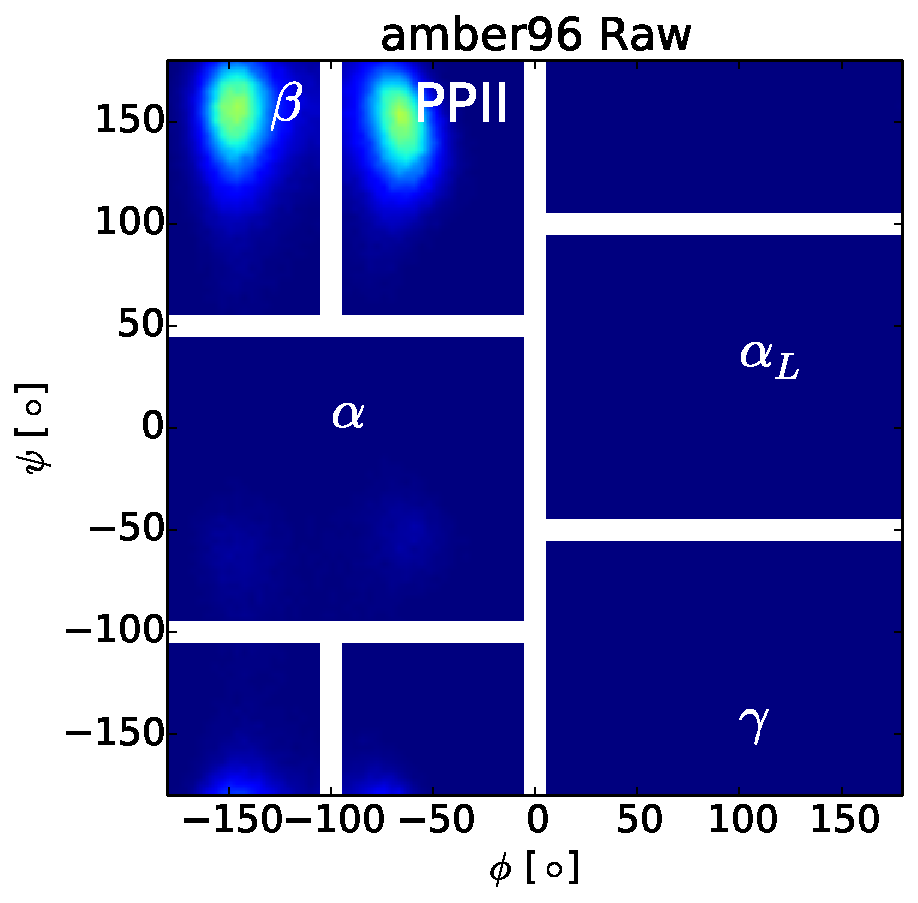
\includegraphics[width=7.05cm]{figures/ALA3_rama_amber96_raw.pdf}
}
\subfigure[]{
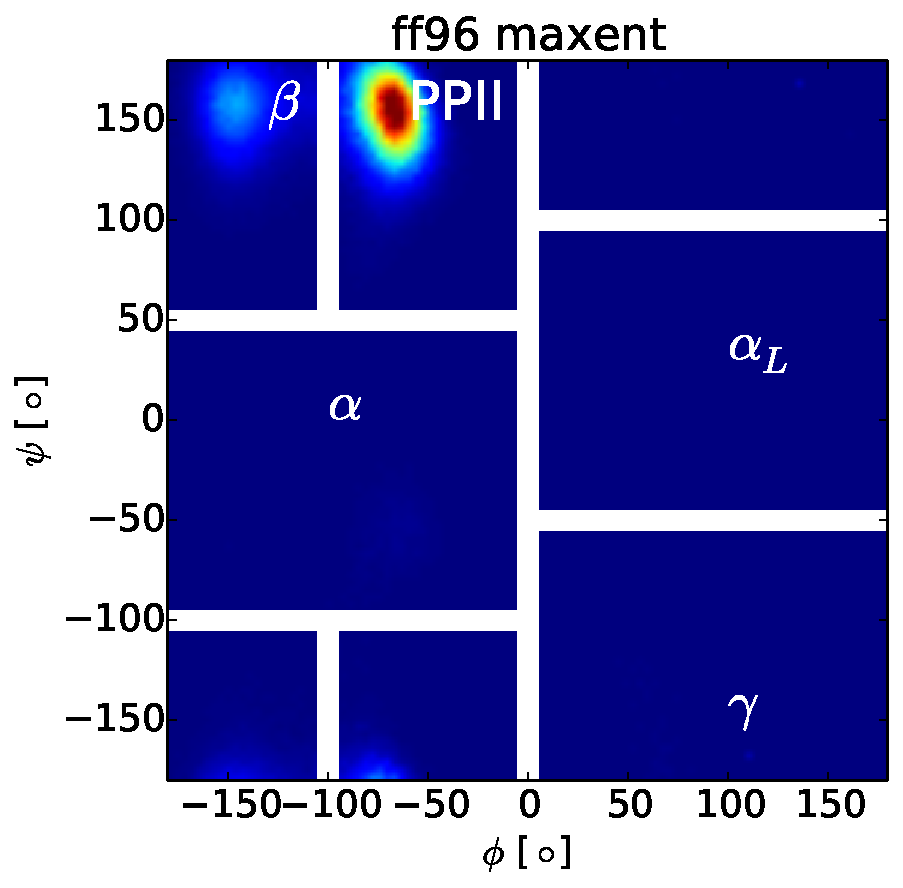
\includegraphics[width=7.05cm]{figures/ALA3_rama_amber96_maxent_belt.pdf}
}

\subfigure[]{
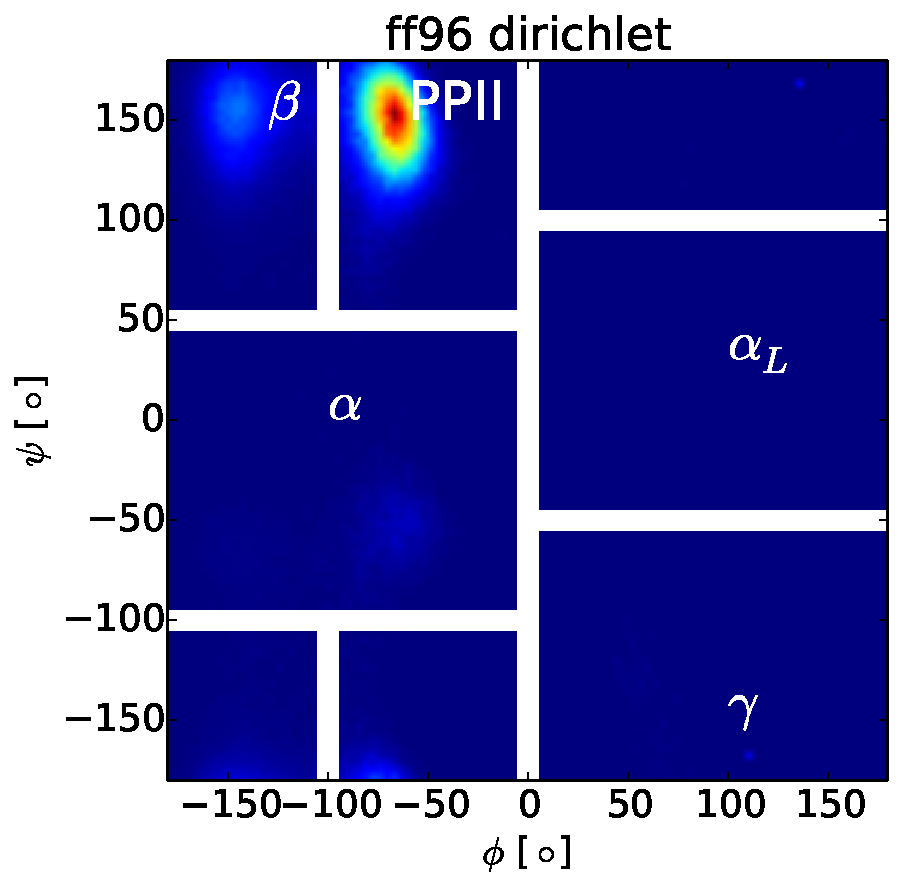
\includegraphics[width=7.05cm]{figures/ALA3_rama_amber96_dirichlet_belt.pdf}
}
\subfigure[]{
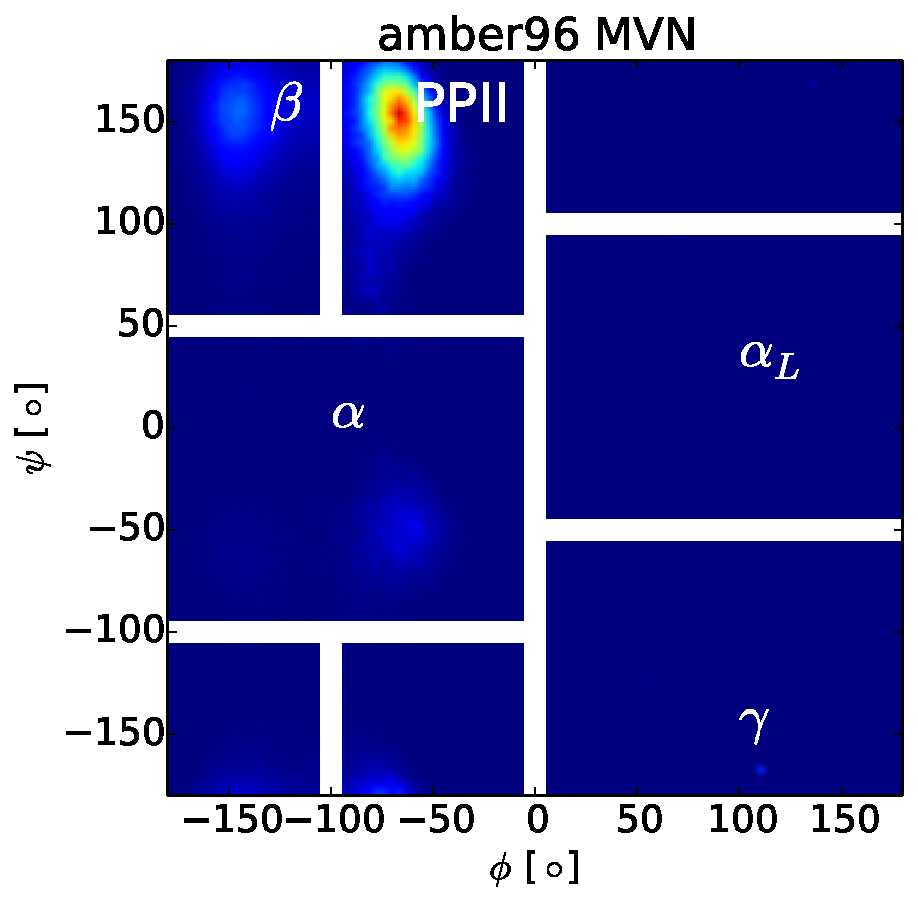
\includegraphics[width=7.05cm]{figures/ALA3_rama_amber96_MVN_belt.pdf}
}

\begin{center}
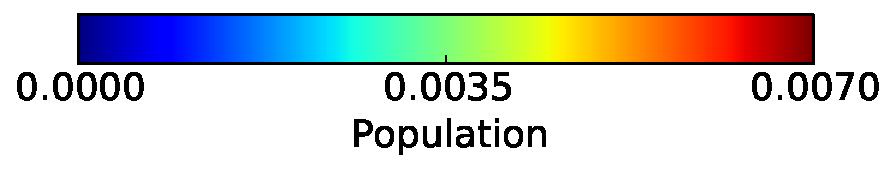
\includegraphics[width=7.05cm]{figures/ALA3_rama_colorbar.pdf}
\end{center}

\end{figure}

\newpage


\begin{figure}
\subfigure[]{
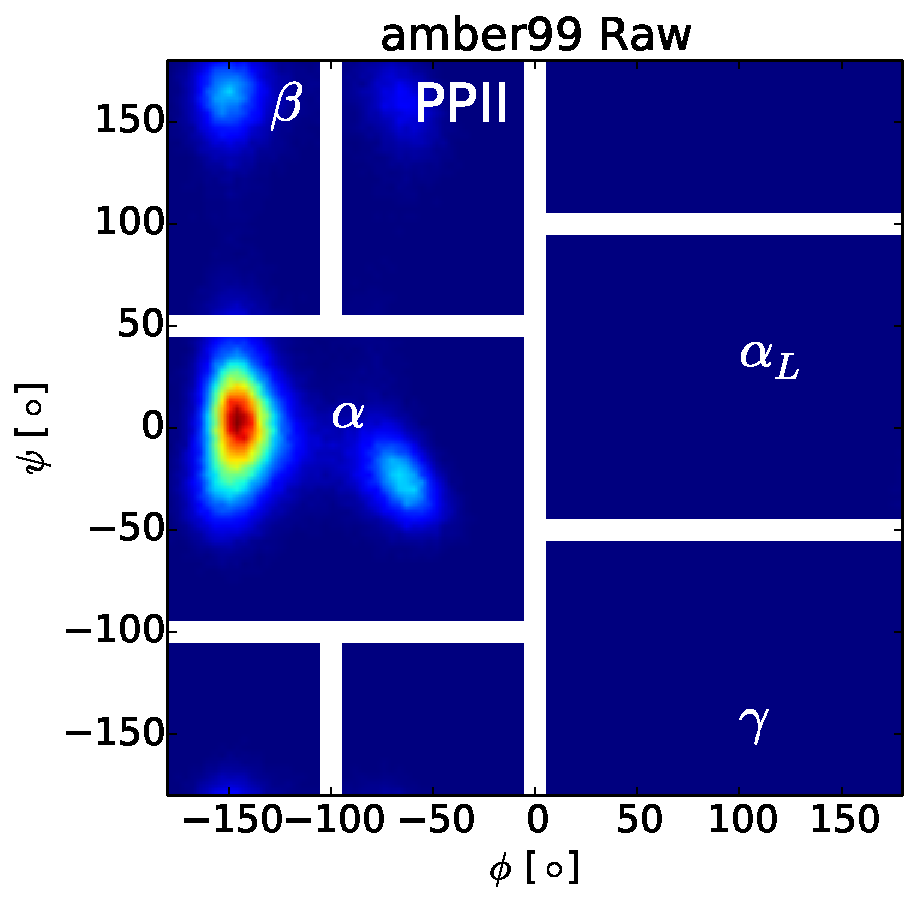
\includegraphics[width=7.05cm]{figures/ALA3_rama_amber99_raw.pdf}
}
\subfigure[]{
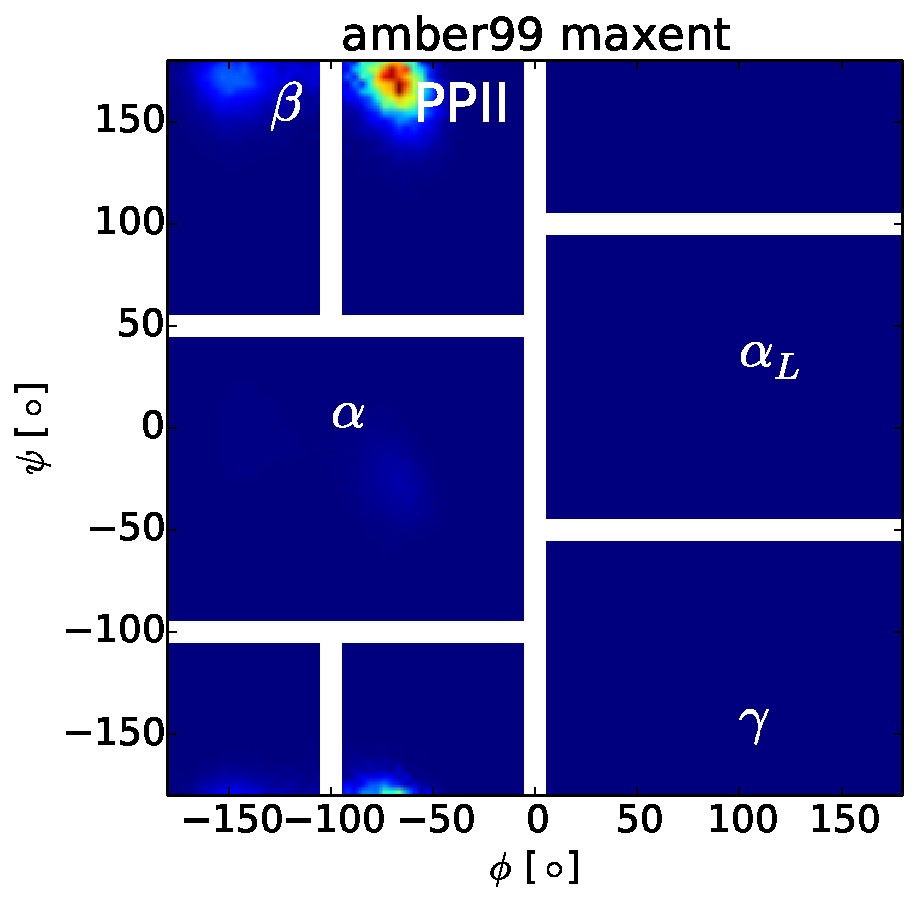
\includegraphics[width=7.05cm]{figures/ALA3_rama_amber99_maxent_belt.pdf}
}

\subfigure[]{
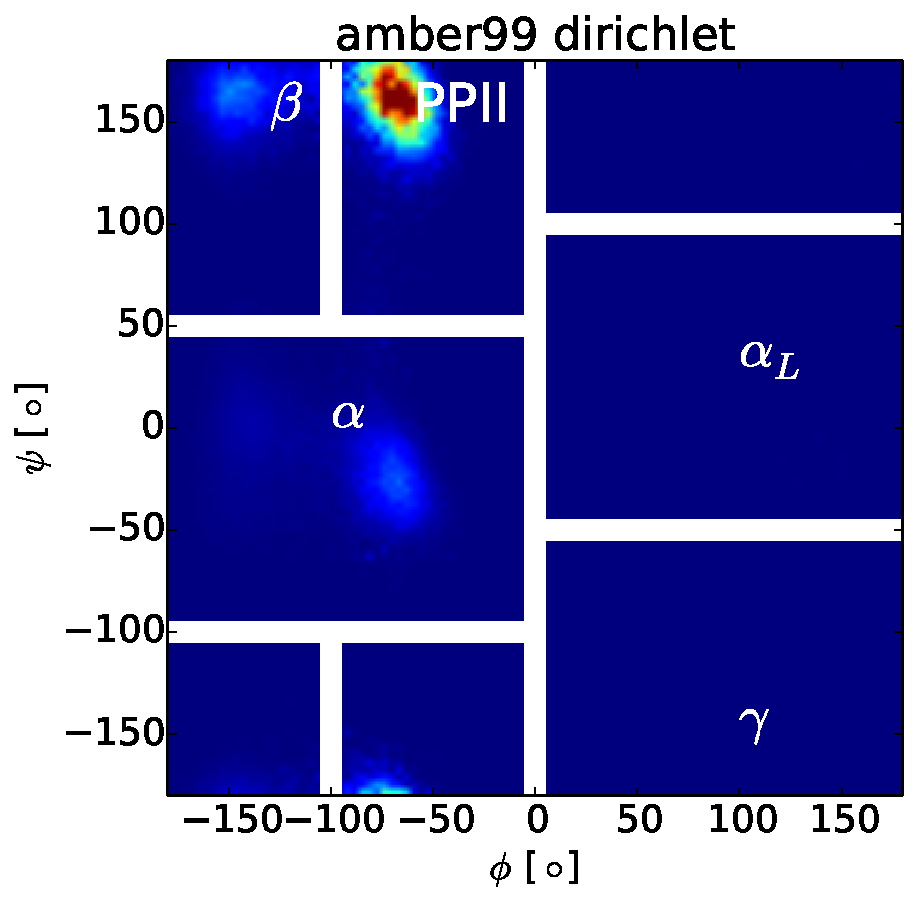
\includegraphics[width=7.05cm]{figures/ALA3_rama_amber99_dirichlet_belt.pdf}
}
\subfigure[]{
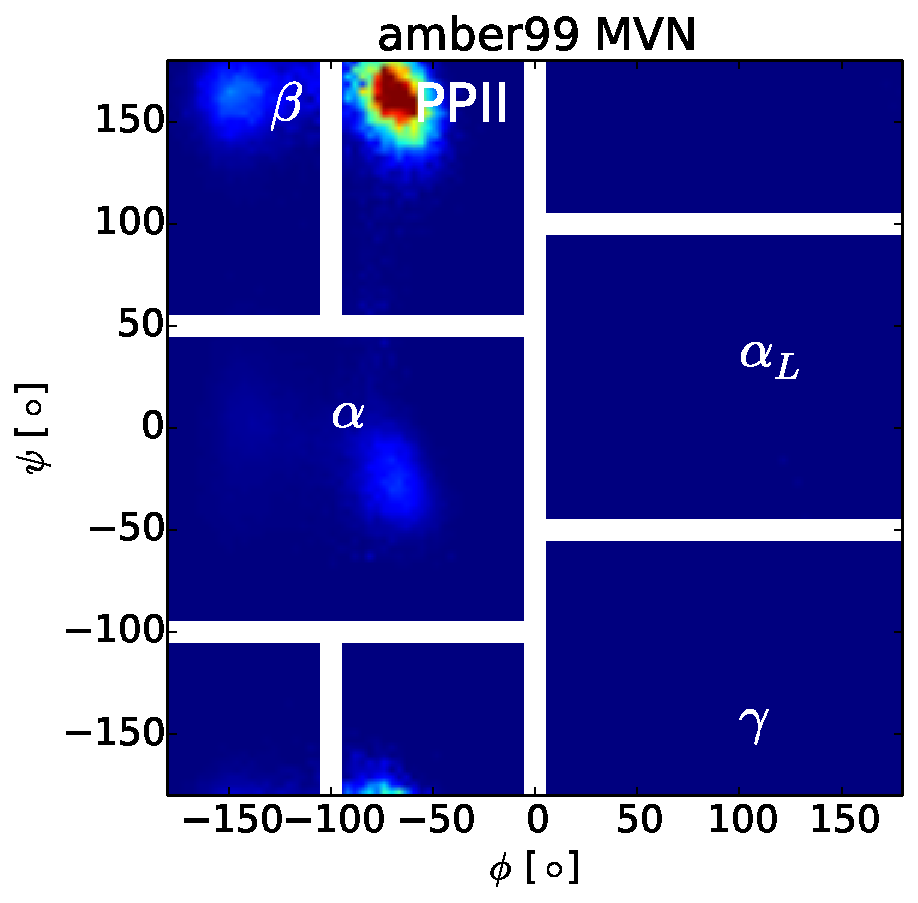
\includegraphics[width=7.05cm]{figures/ALA3_rama_amber99_MVN_belt.pdf}
}

\begin{center}
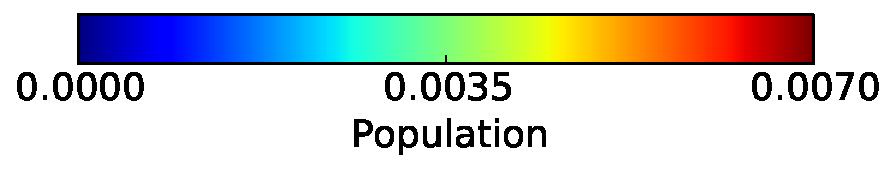
\includegraphics[width=7.05cm]{figures/ALA3_rama_colorbar.pdf}
\end{center}

\end{figure}

\newpage

\begin{figure}
\subfigure[]{
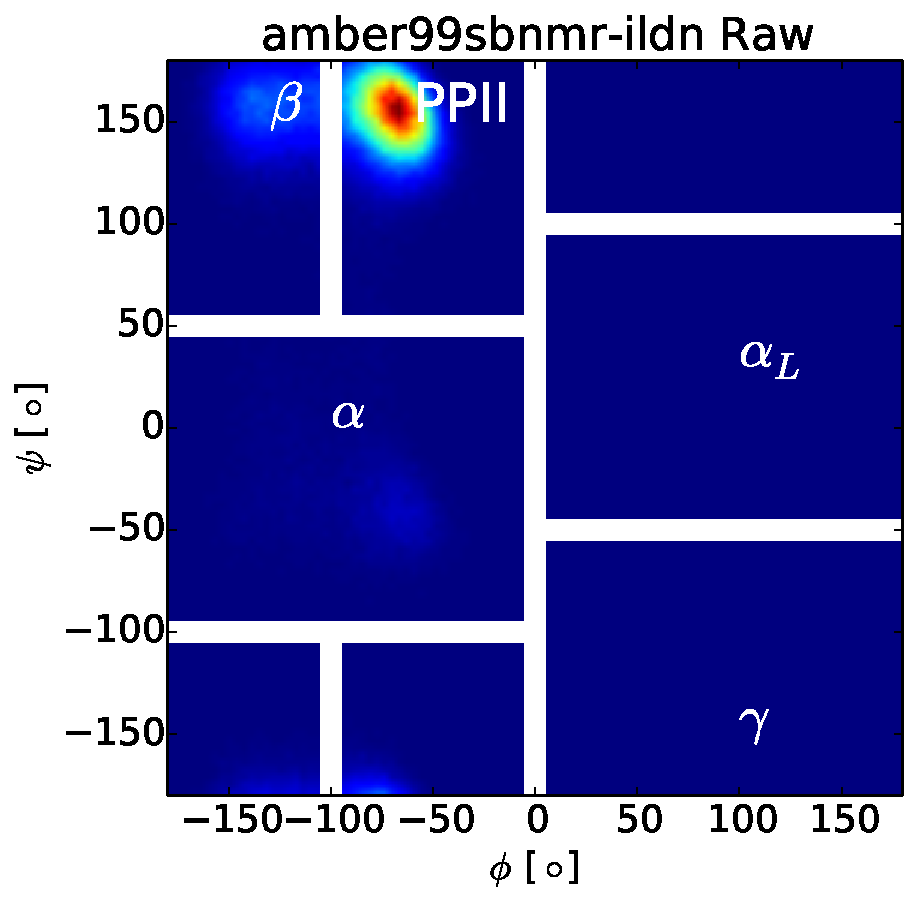
\includegraphics[width=7.05cm]{figures/ALA3_rama_amber99sbnmr-ildn_raw.pdf}
}
\subfigure[]{
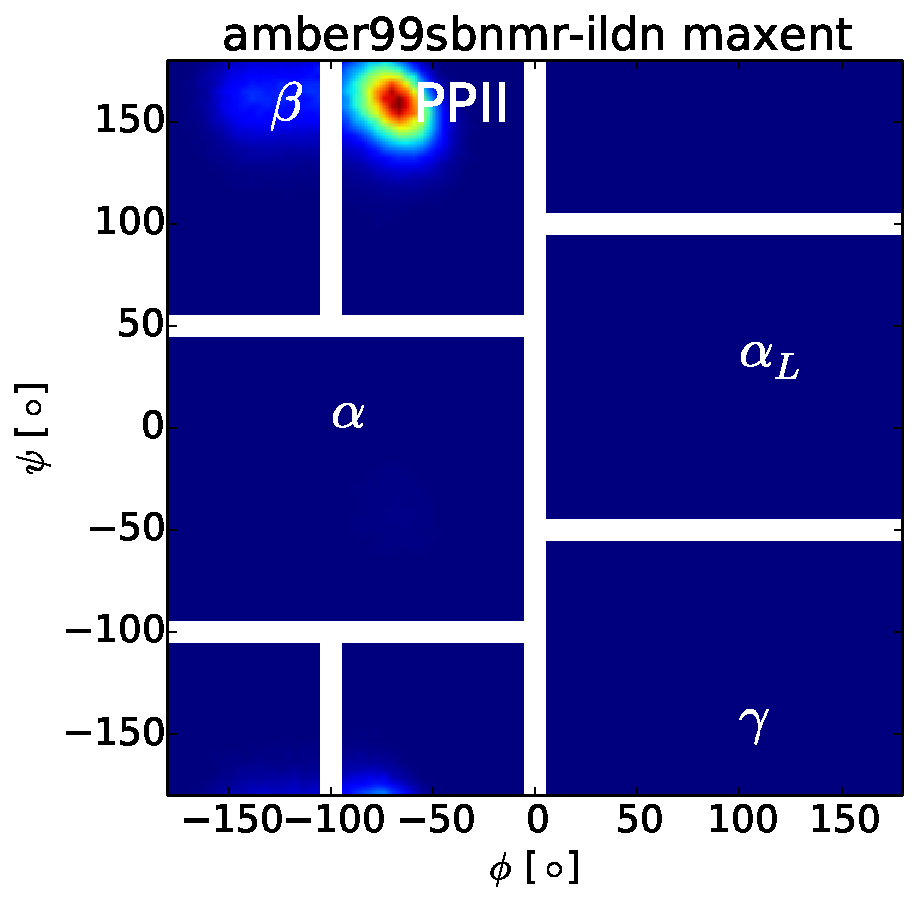
\includegraphics[width=7.05cm]{figures/ALA3_rama_amber99sbnmr-ildn_maxent_belt.pdf}
}

\subfigure[]{
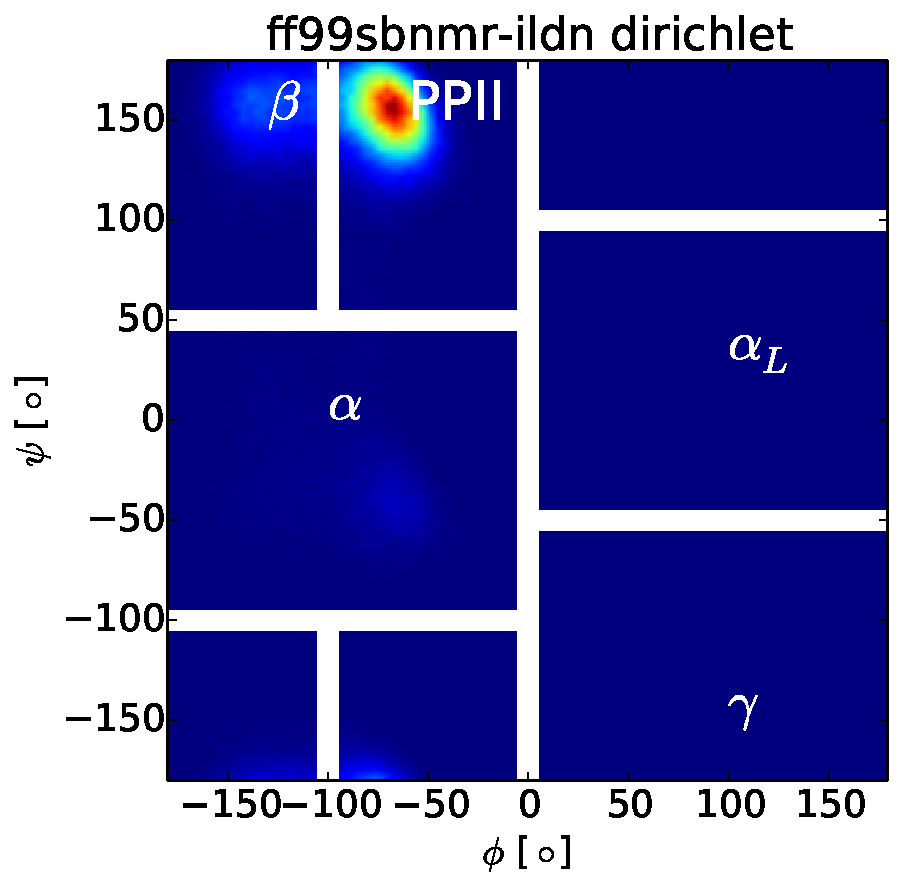
\includegraphics[width=7.05cm]{figures/ALA3_rama_amber99sbnmr-ildn_dirichlet_belt.pdf}
}
\subfigure[]{
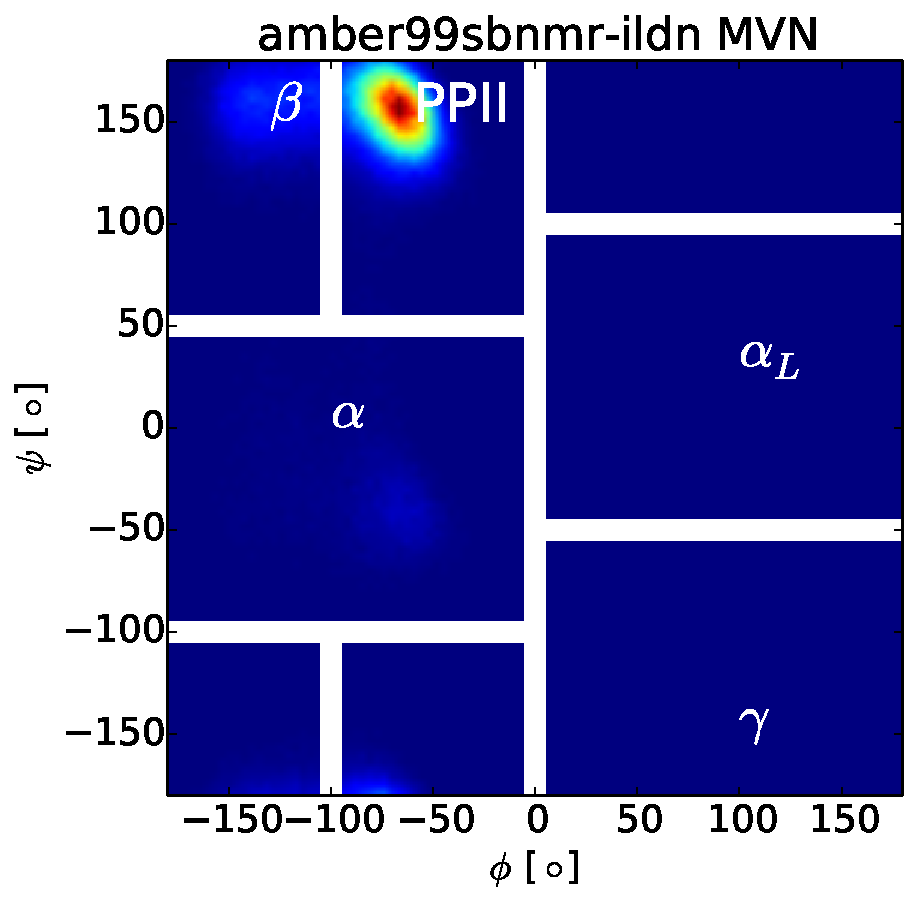
\includegraphics[width=7.05cm]{figures/ALA3_rama_amber99sbnmr-ildn_MVN_belt.pdf}
}

\begin{center}
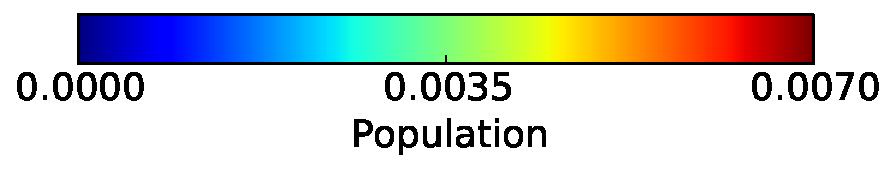
\includegraphics[width=7.05cm]{figures/ALA3_rama_colorbar.pdf}
\end{center}

\end{figure}

\newpage

\begin{figure}
\subfigure[]{
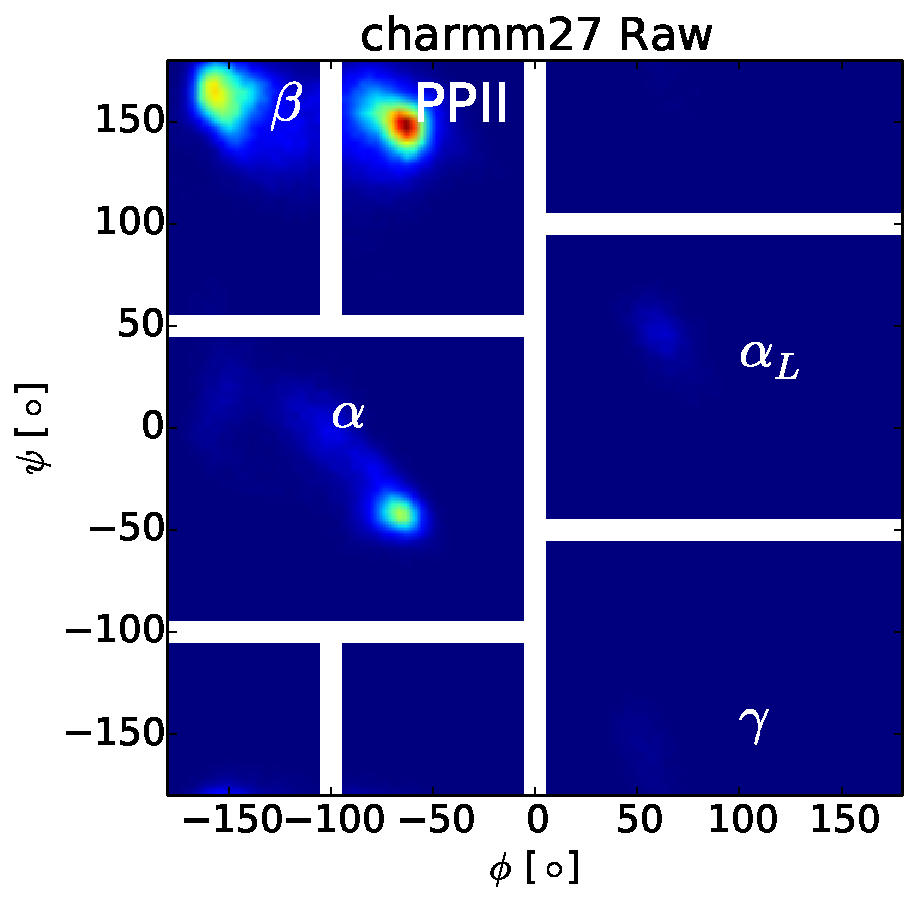
\includegraphics[width=7.05cm]{figures/ALA3_rama_charmm27_raw.pdf}
}
\subfigure[]{
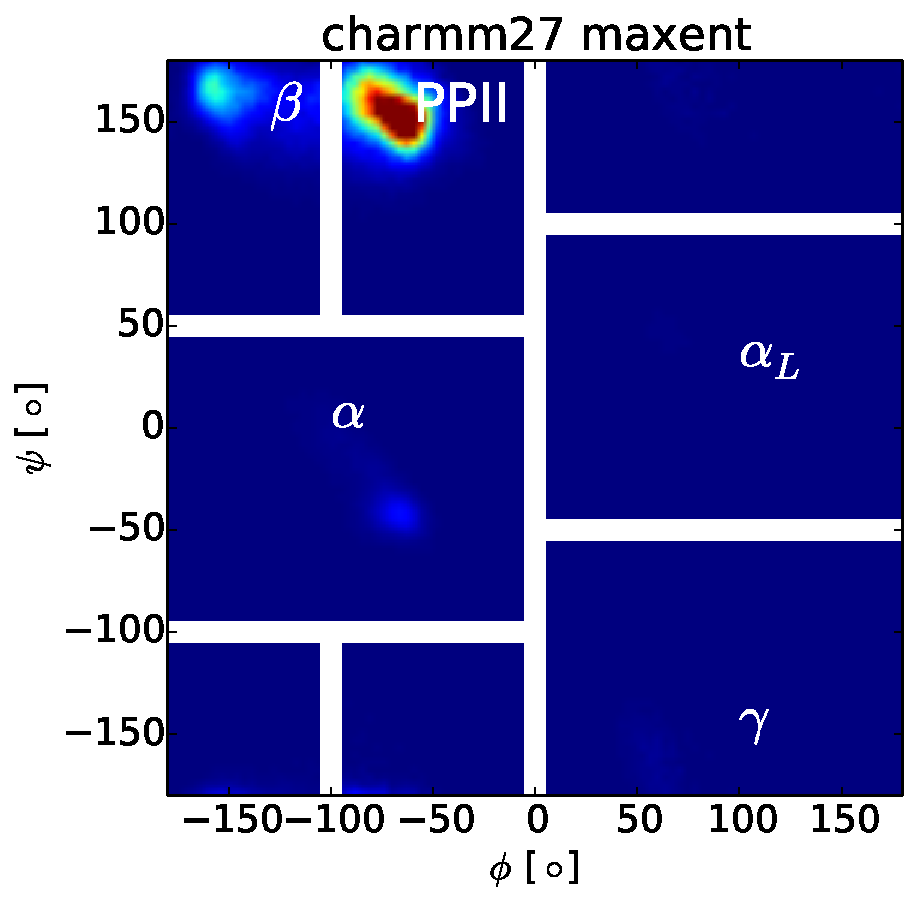
\includegraphics[width=7.05cm]{figures/ALA3_rama_charmm27_maxent_belt.pdf}
}

\subfigure[]{
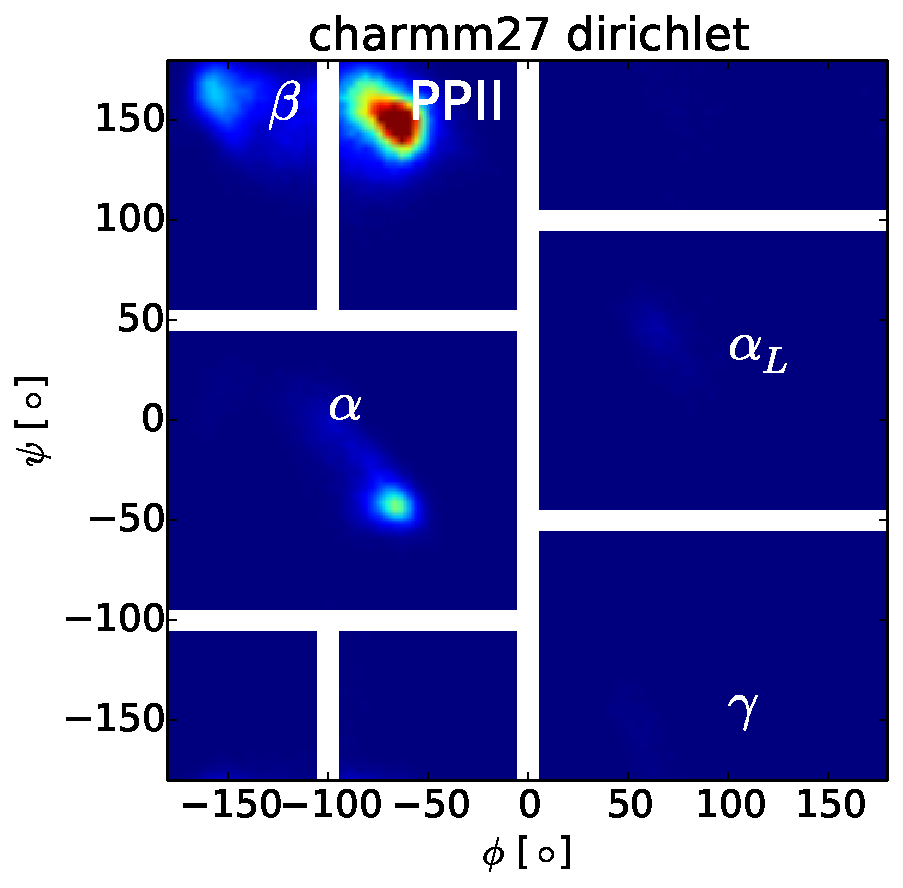
\includegraphics[width=7.05cm]{figures/ALA3_rama_charmm27_dirichlet_belt.pdf}
}
\subfigure[]{
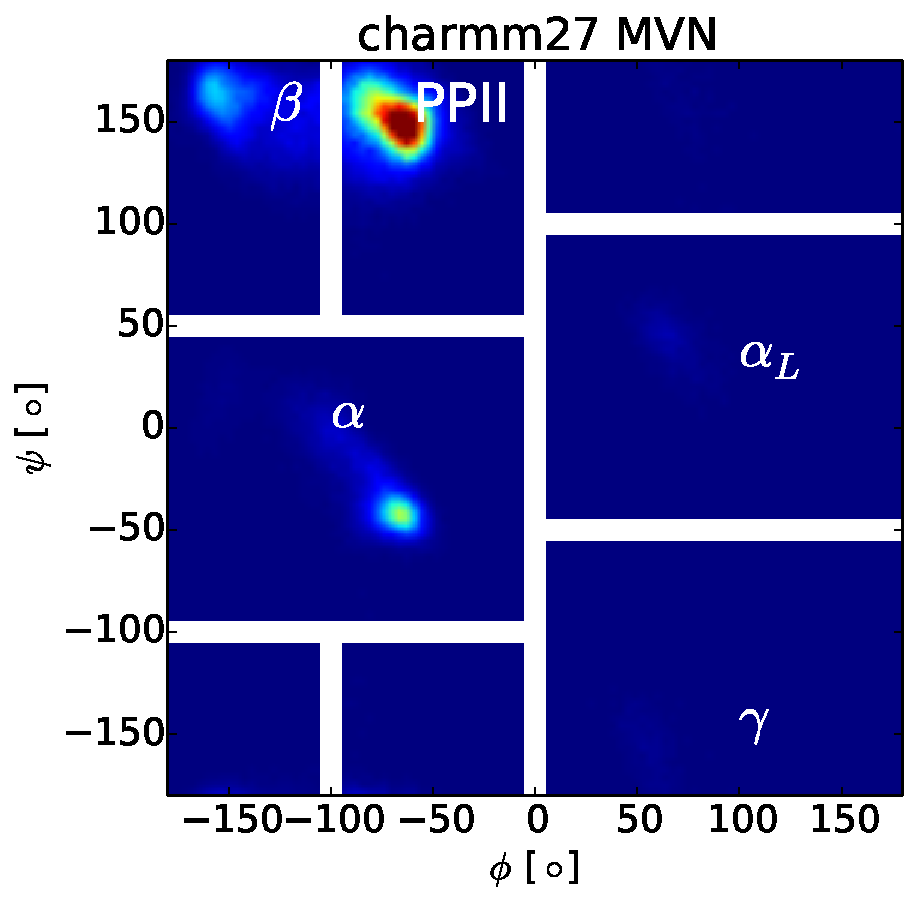
\includegraphics[width=7.05cm]{figures/ALA3_rama_charmm27_MVN_belt.pdf}
}

\begin{center}
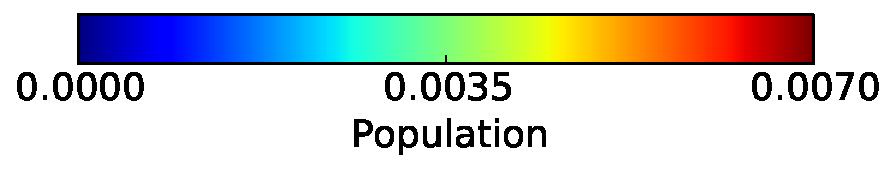
\includegraphics[width=7.05cm]{figures/ALA3_rama_colorbar.pdf}
\end{center}

\end{figure}

\newpage

\begin{figure}
\subfigure[]{
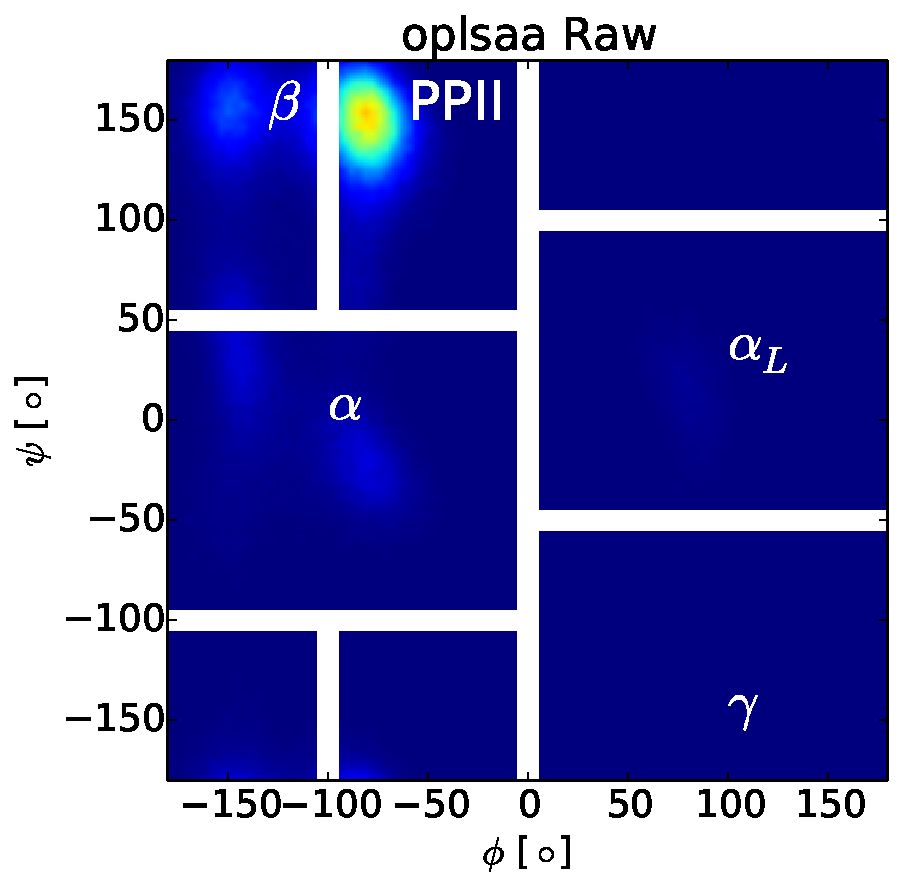
\includegraphics[width=7.05cm]{figures/ALA3_rama_oplsaa_raw.pdf}
}
\subfigure[]{
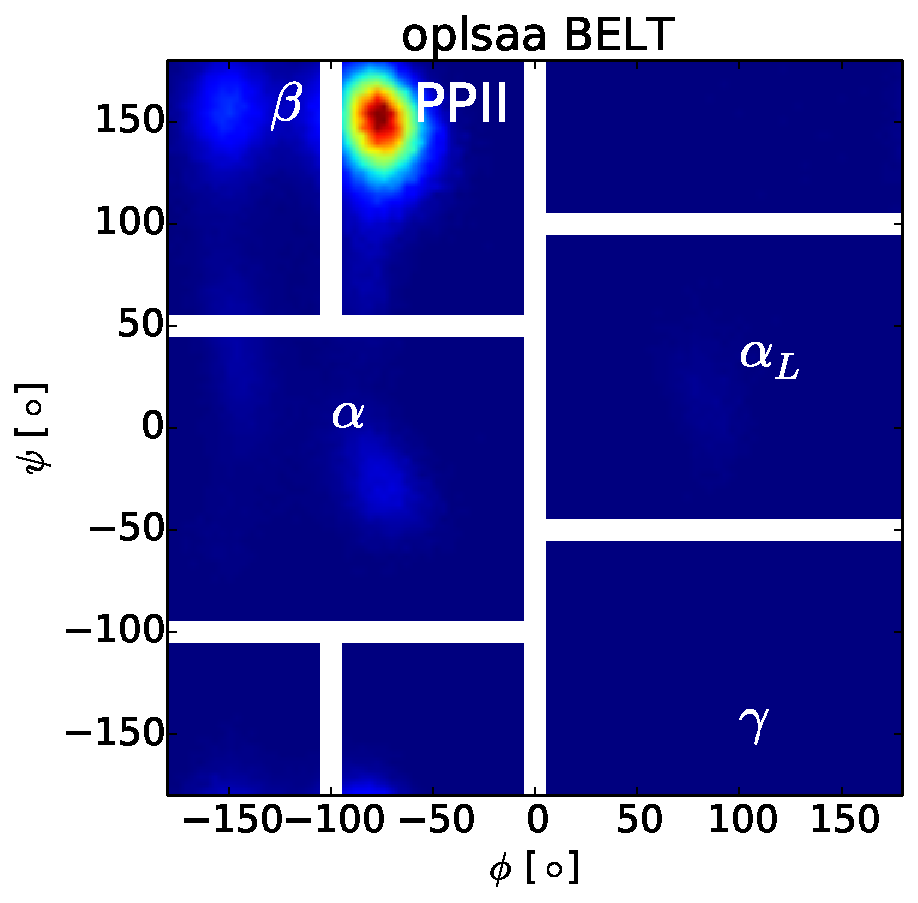
\includegraphics[width=7.05cm]{figures/ALA3_rama_oplsaa_maxent_belt.pdf}
}

\subfigure[]{
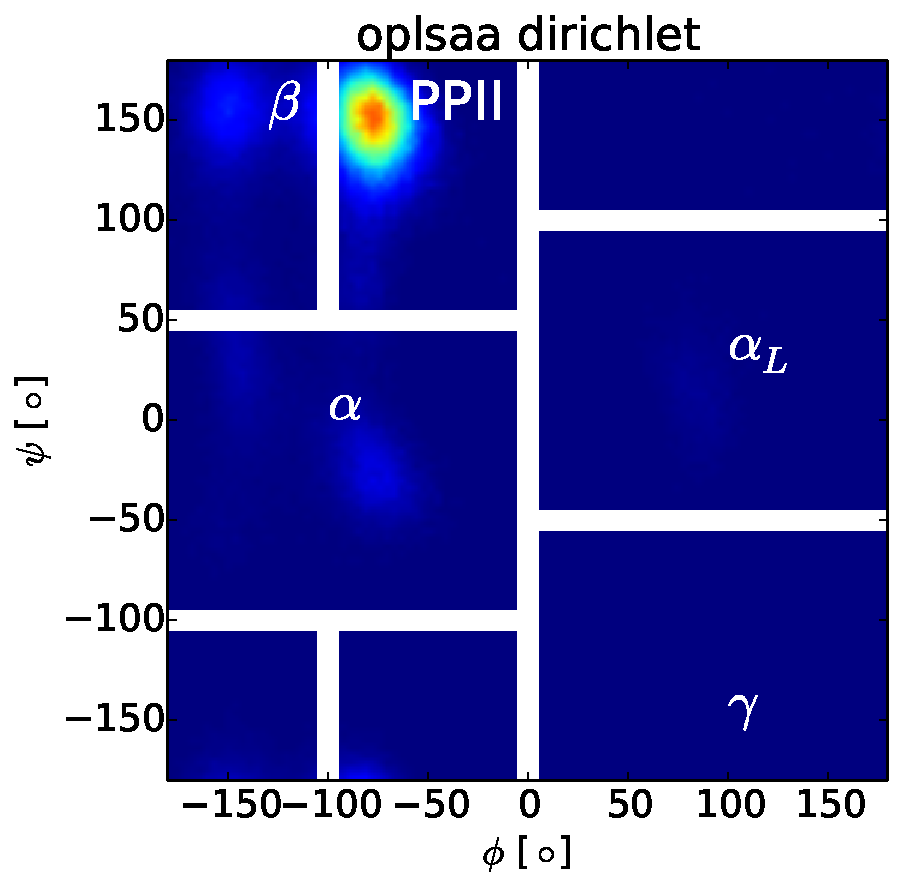
\includegraphics[width=7.05cm]{figures/ALA3_rama_oplsaa_dirichlet_belt.pdf}
}
\subfigure[]{
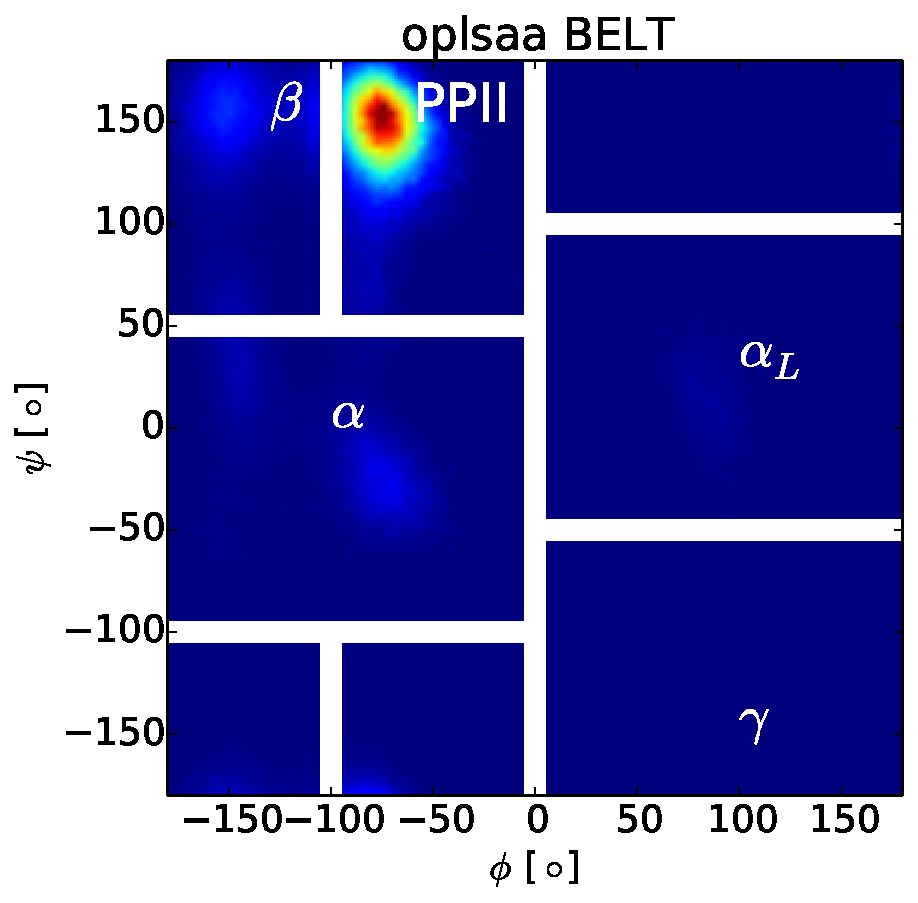
\includegraphics[width=7.05cm]{figures/ALA3_rama_oplsaa_MVN_belt.pdf}
}

\begin{center}
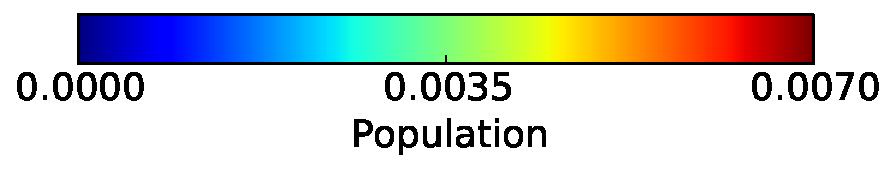
\includegraphics[width=7.05cm]{figures/ALA3_rama_colorbar.pdf}
\end{center}

\caption{
Ramachandran plots (2D histograms) of MD simulations and BELT models.  
}
\label{figure:test}


\end{figure}

\newpage


\begin{figure}
\subfigure[]{
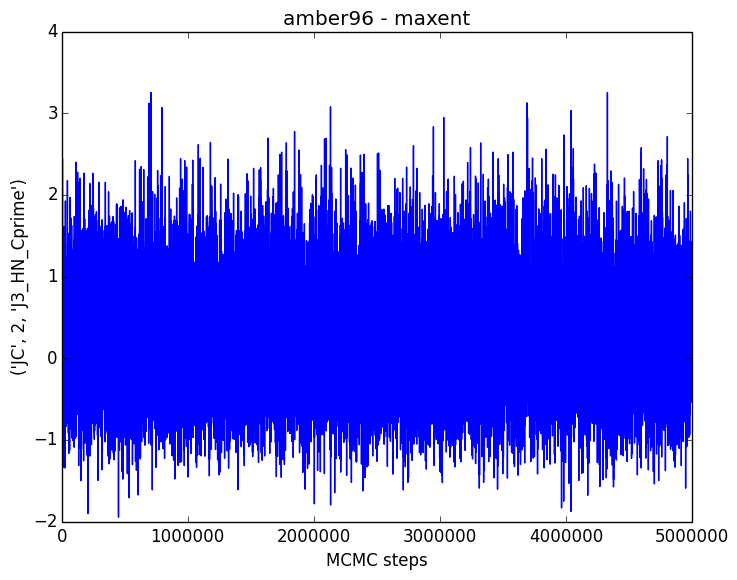
\includegraphics[width=7.5cm]{figures/maxent-amber96-MCMC_Trace.png}
}
\subfigure[]{
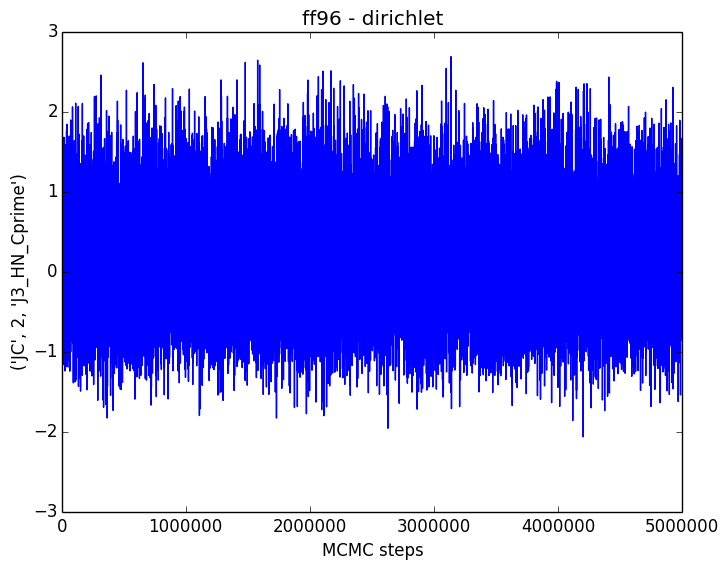
\includegraphics[width=7.5cm]{figures/dirichlet-amber96-MCMC_Trace.png}
}

\subfigure[]{
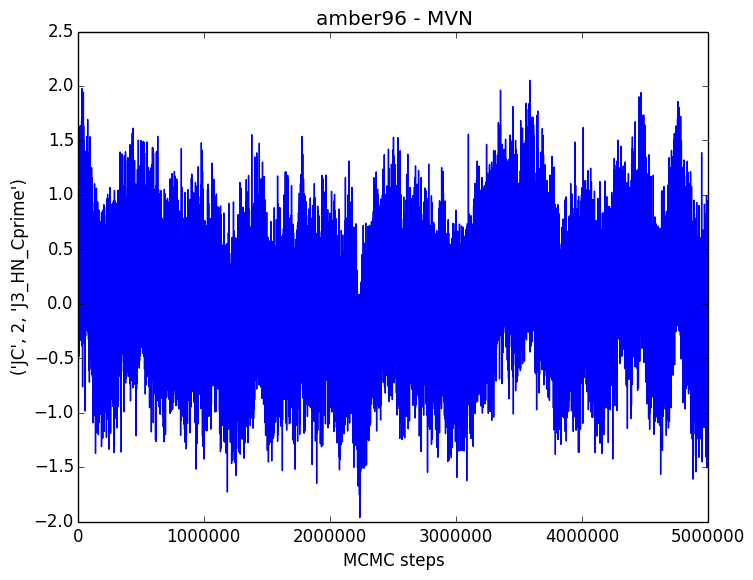
\includegraphics[width=7.5cm]{figures/MVN-amber96-MCMC_Trace.png}
}
\end{figure}

\newpage

\begin{figure}
\subfigure[]{
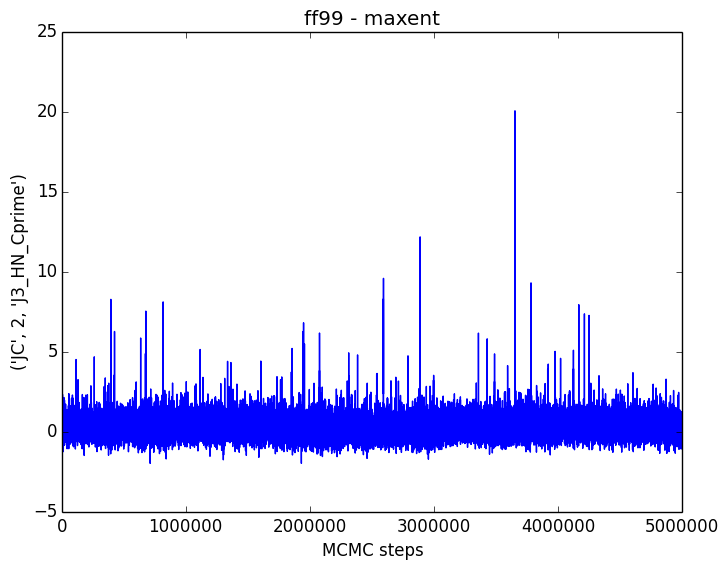
\includegraphics[width=7.5cm]{figures/maxent-amber99-MCMC_Trace.png}
}
\subfigure[]{
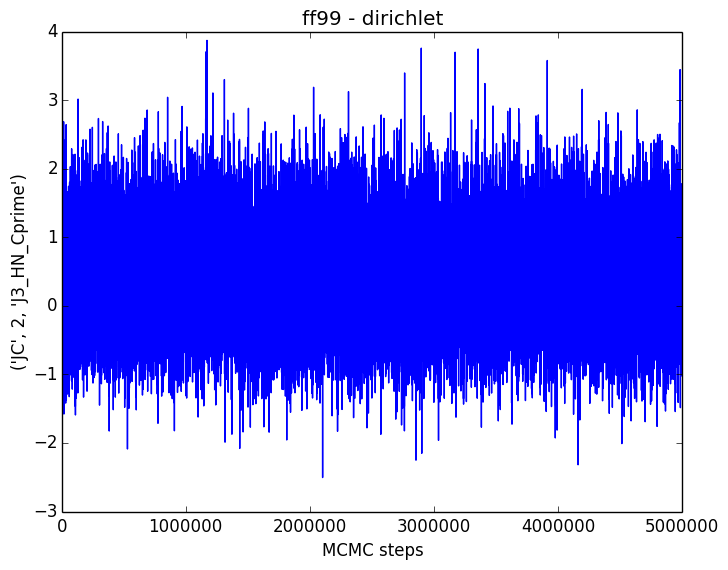
\includegraphics[width=7.5cm]{figures/dirichlet-amber99-MCMC_Trace.png}
}

\subfigure[]{
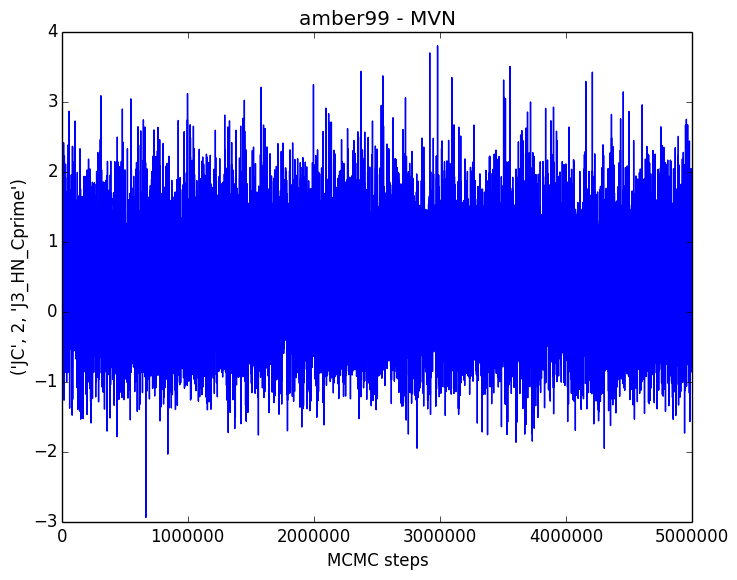
\includegraphics[width=7.5cm]{figures/MVN-amber99-MCMC_Trace.png}
}
\end{figure}

\newpage

\begin{figure}
\subfigure[]{
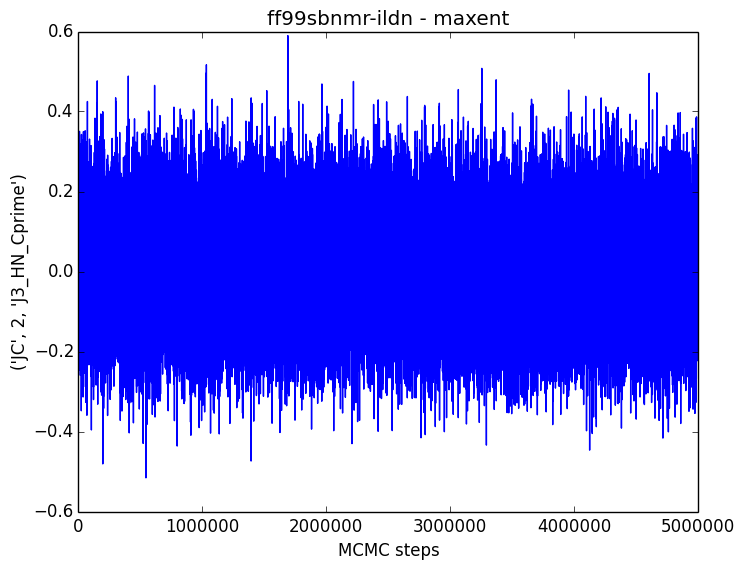
\includegraphics[width=7.5cm]{figures/maxent-amber99sbnmr-ildn-MCMC_Trace.png}
}
\subfigure[]{
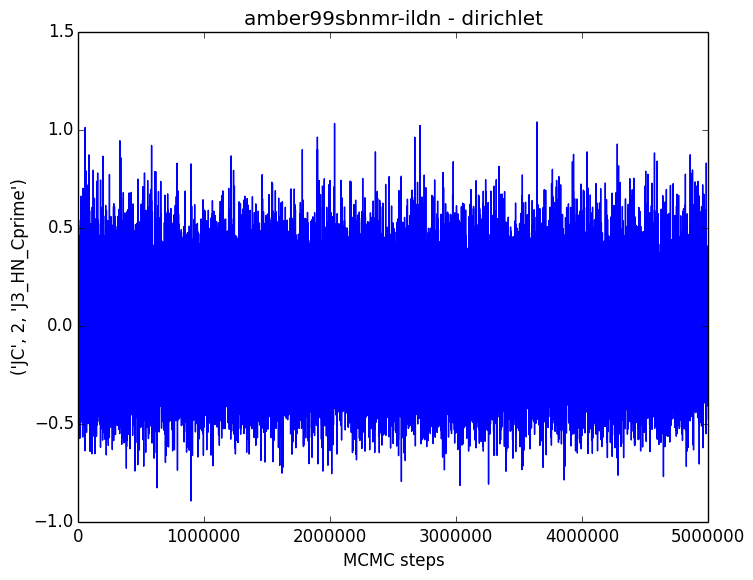
\includegraphics[width=7.5cm]{figures/dirichlet-amber99sbnmr-ildn-MCMC_Trace.png}
}

\subfigure[]{
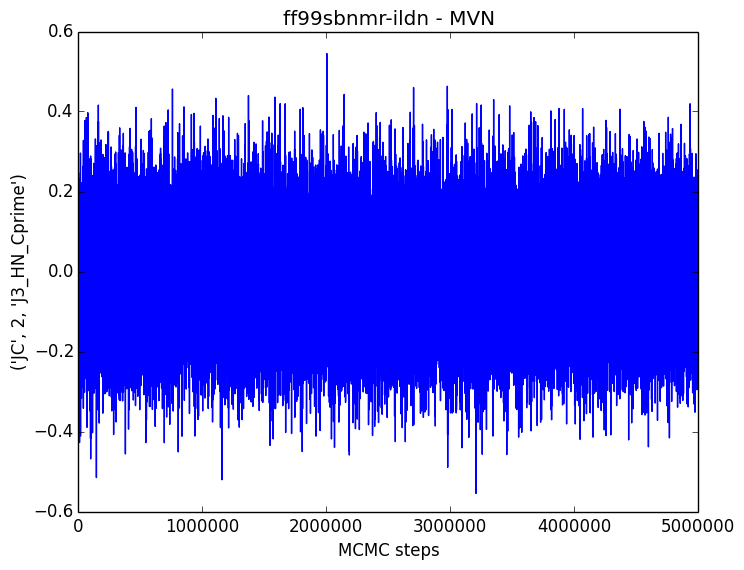
\includegraphics[width=7.5cm]{figures/MVN-amber99sbnmr-ildn-MCMC_Trace.png}
}
\end{figure}

\newpage

\begin{figure}
\subfigure[]{
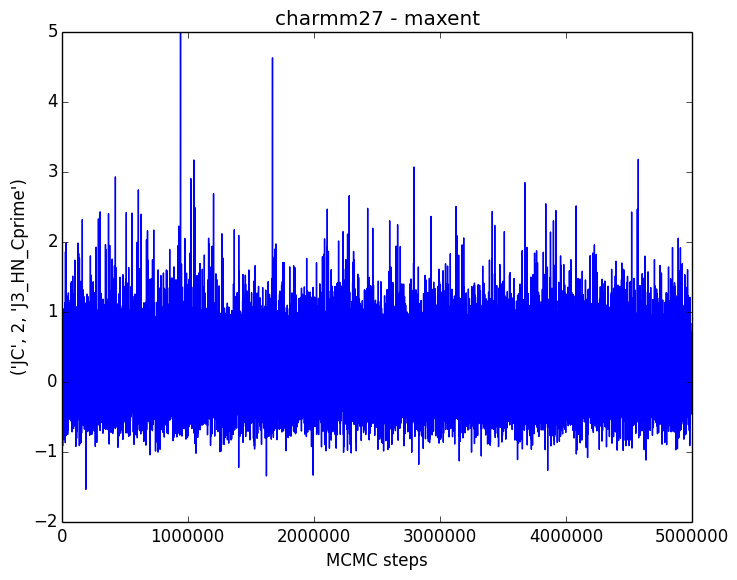
\includegraphics[width=7.5cm]{figures/maxent-charmm27-MCMC_Trace.png}
}
\subfigure[]{
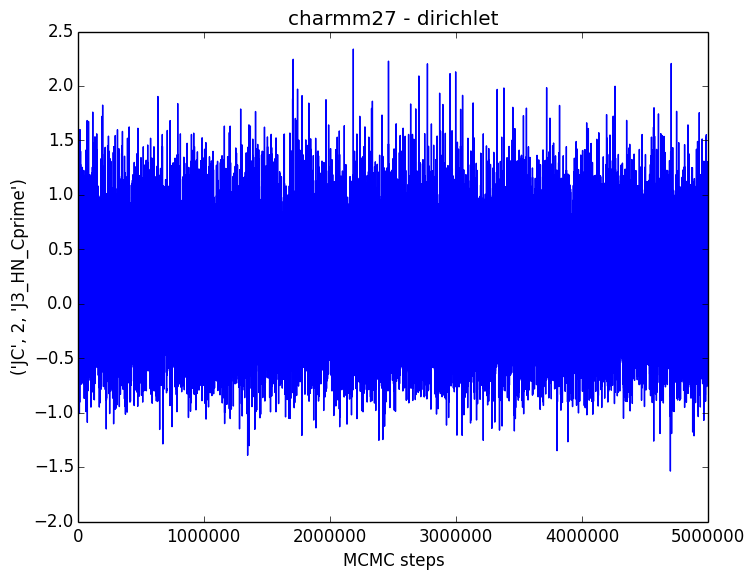
\includegraphics[width=7.5cm]{figures/dirichlet-charmm27-MCMC_Trace.png}
}

\subfigure[]{
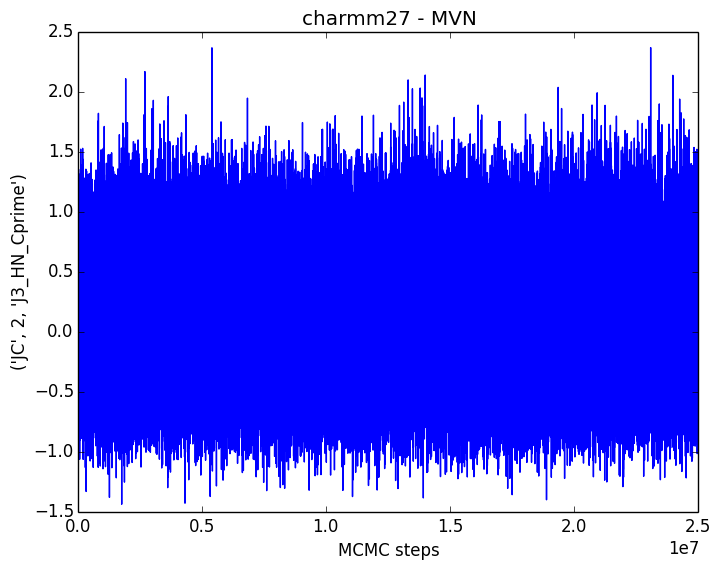
\includegraphics[width=7.5cm]{figures/MVN-charmm27-MCMC_Trace.png}
}
\end{figure}

\newpage

\begin{figure}
\subfigure[]{
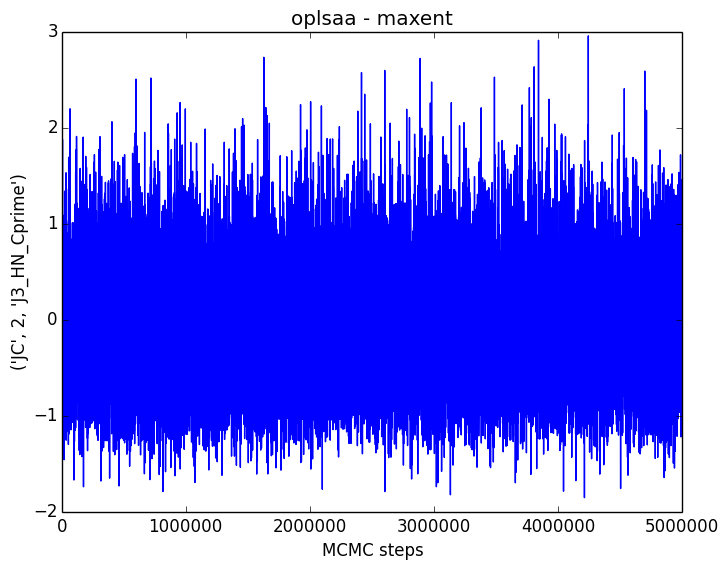
\includegraphics[width=7.5cm]{figures/maxent-oplsaa-MCMC_Trace.png}
}
\subfigure[]{
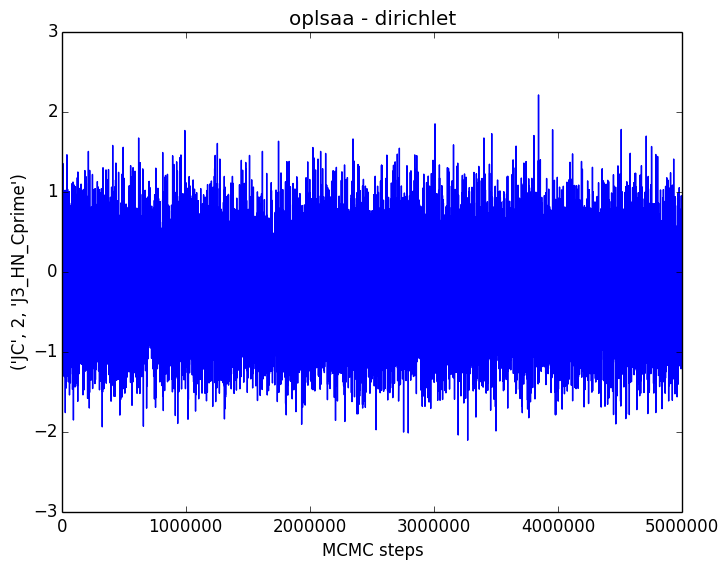
\includegraphics[width=7.5cm]{figures/dirichlet-oplsaa-MCMC_Trace.png}
}

\subfigure[]{
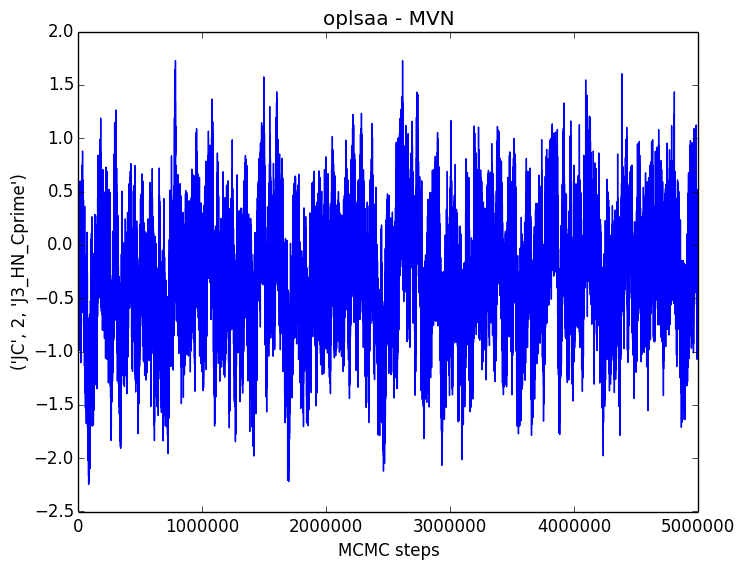
\includegraphics[width=7.5cm]{figures/MVN-oplsaa-MCMC_Trace.png}
}

\caption{
MCMC traces of first component of $\alpha$.  
}
\label{figure:MCMC}
\end{figure}

\newpage

\begin{figure}
\subfigure[]{
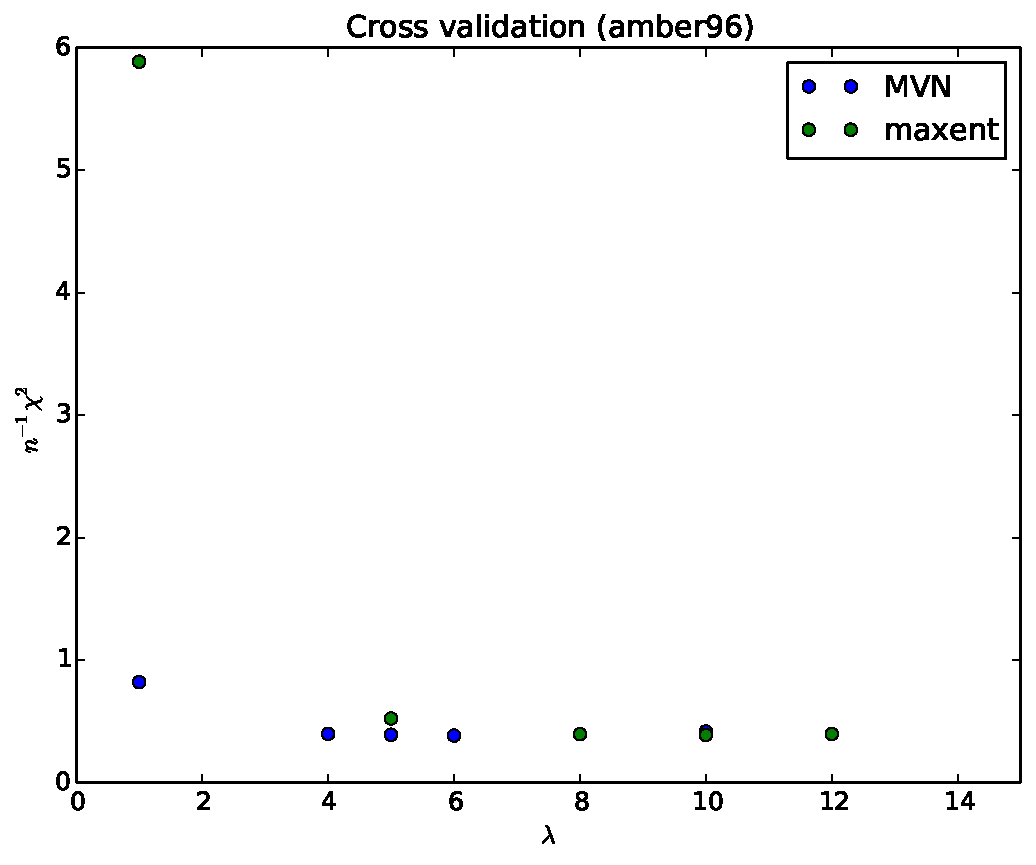
\includegraphics[width=7.5cm]{figures/cross_val_amber96.pdf}
}
\subfigure[]{
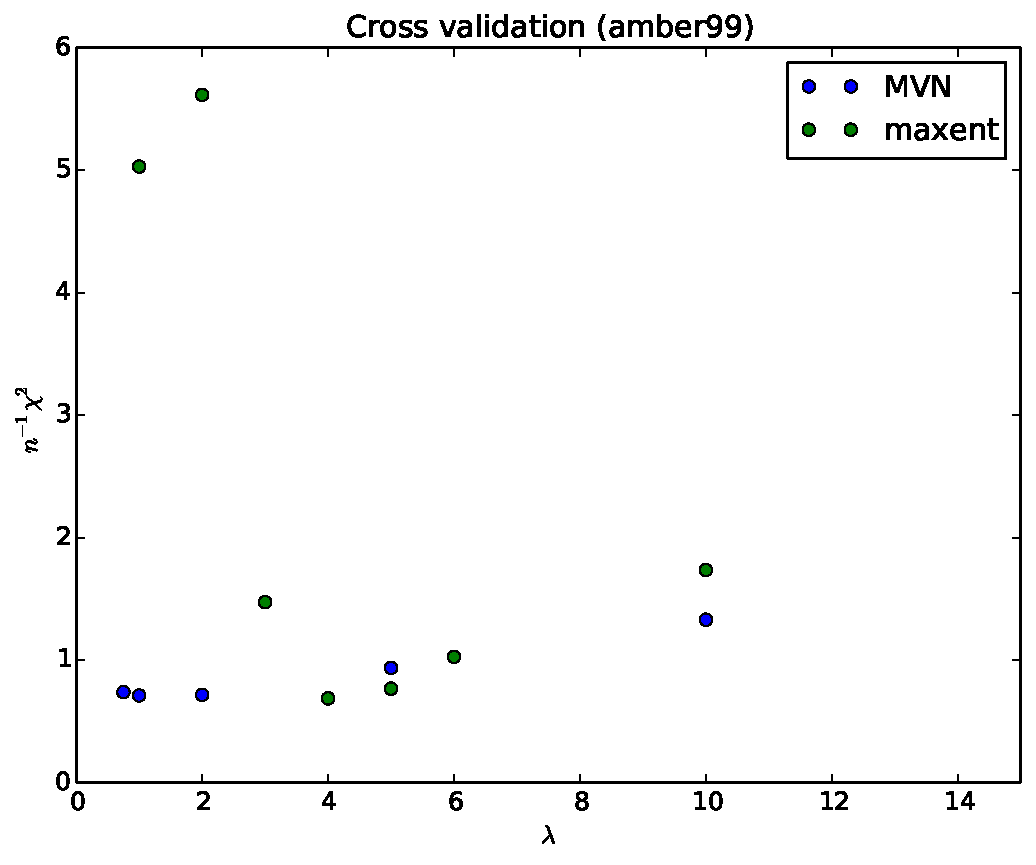
\includegraphics[width=7.5cm]{figures/cross_val_amber99.pdf}
}

\subfigure[]{
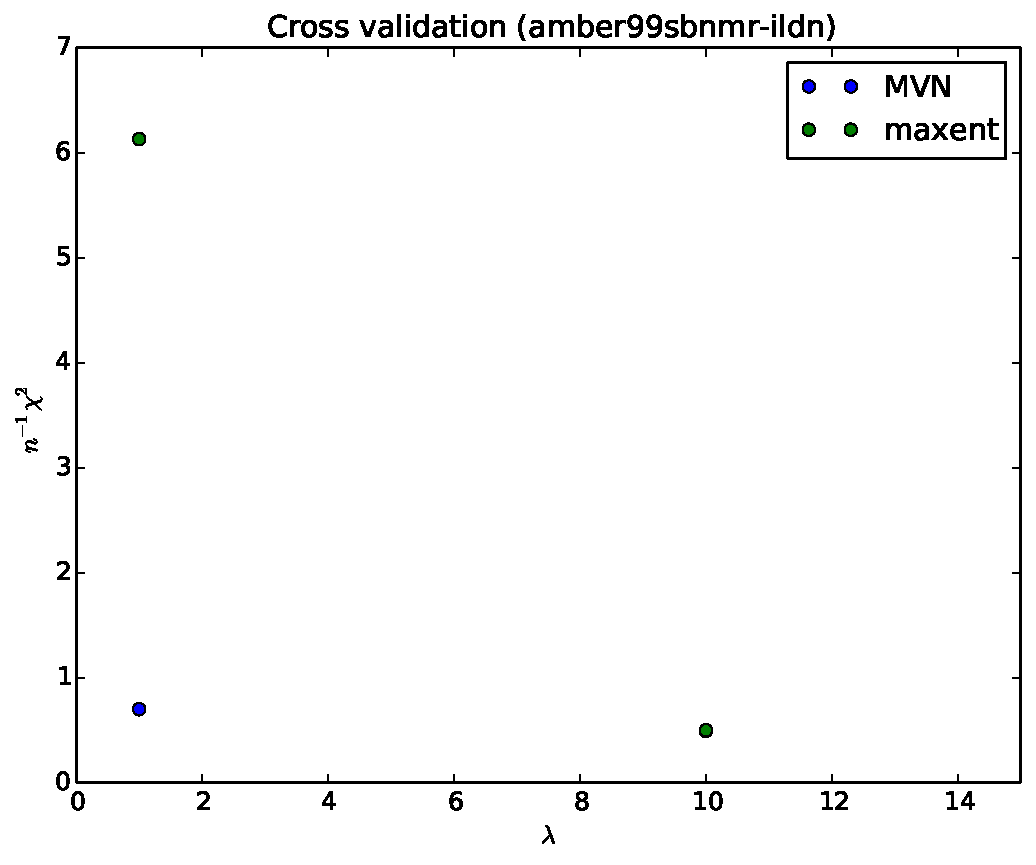
\includegraphics[width=7.5cm]{figures/cross_val_amber99sbnmr-ildn.pdf}
}

\subfigure[]{
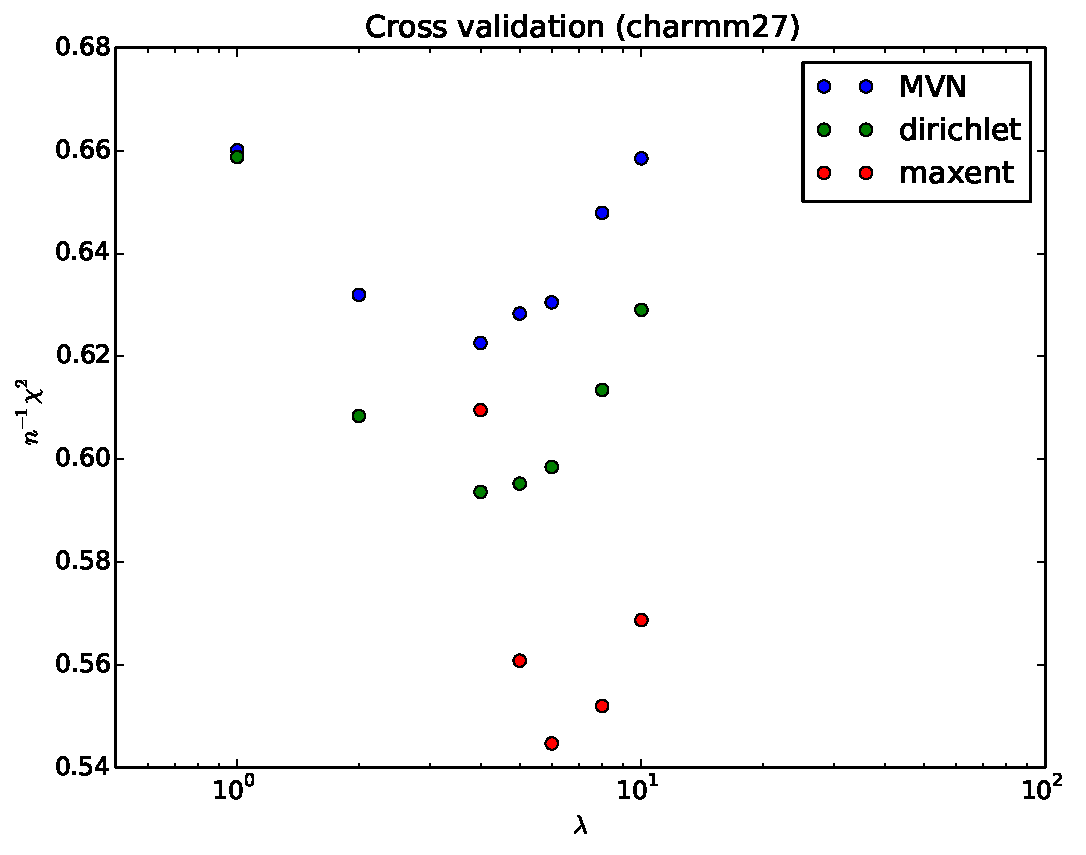
\includegraphics[width=7.5cm]{figures/cross_val_charmm27.pdf}
}
\subfigure[]{
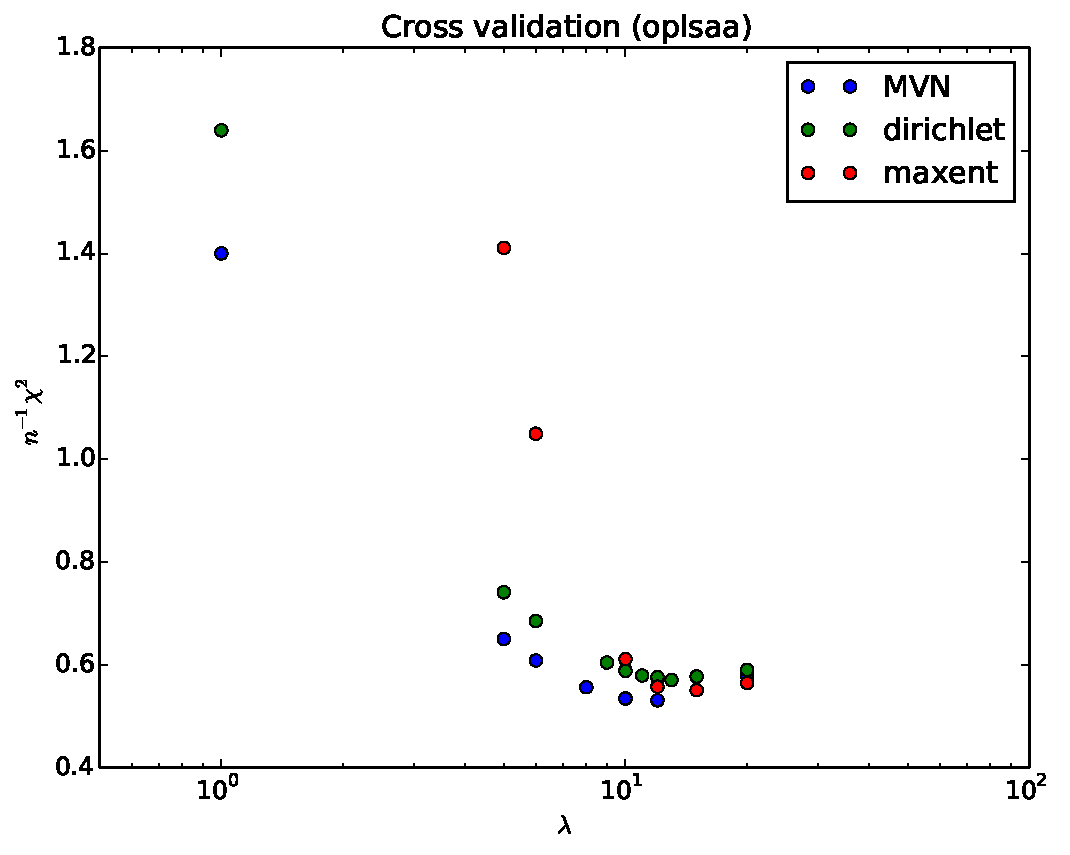
\includegraphics[width=7.5cm]{figures/cross_val_oplsaa.pdf}
}

\caption{
Cross validated reduced $\chi^2$.  Cross validation was performed using twenty-fold subsampled trajectory data to make calculations computationally tractable.  
}
\label{figure:cross_val}
\end{figure}


\clearpage

\section*{Appendix S1.  Connecting BELT, Maximum Entropy, and Hyperensembles}

Bayesian Energy Landscape Tilting generalizes a recent maximum entropy formalism \cite{chodera2012} to include statistical uncertainty.  Here, we outline the previous results and detail the connection between BELT and the previous maximum entropy formalism.  We also show how a hyperensemble formalism of Crooks \cite{crooks2007beyond} naturally leads to BELT-like models.

\subsection*{Outline of Maximum Entropy Formalism}

The previous work \cite{chodera2012} used Jaynes' maximum entropy arguments \cite{jaynes1957information} to derive a new approach to constraining simulations.  Here we outline those arguments for the case of a single observable.  

The maximum entropy formalism relies on finding the least informative probability distribution that is compatible with some known constraints.  The information entropy is used as the metric for quantifying the information content of a distribution:

$$S(p) = - \int p(x) \log(p(x)) dx $$

The method of Chodera and Pitera uses three constraints on $p(x)$.  First, $p(x)$ must be a well-defined probability distribution:

$$\int p(x) dx = 1 $$

Second, $p(x)$ must give the correct average potential energy:

$$\int U(x) p(x) dx = \frac{3}{2} N k_B T$$

Finally, we assume that we have access to an ensemble-average measurement $F$ and a function $f(x)$ that predicts the observable as a function of atomic coordinates:

$$\int f(x) p(x) dx = F$$

This constrained optimization problem is solved via Lagrange multipliers, eventually leading to the following gradient condition:

$$\frac{\partial S}{\partial p} - \lambda_0 \frac{\partial g_0}{\partial p}- \lambda_1 \frac{\partial g_1}{\partial p}- \lambda_2 \frac{\partial g_2}{\partial p} = 0$$

Here, the functions $g_0$, $g_1$, and $g_2$ are the following constraint equations:

$$g_0 = \int dx p(x) - 1$$

$$g_1 = \int dx U(x) p(x) - \frac{3}{2} N K_B T$$

$$g_2 = \int dx f(x) p(x) - F$$

The solution to this optimization problem is given by 

$$p(x) \propto \exp(-\beta U(x) + \alpha f(x))$$

Sampling the potential $U(x) + \alpha f(x)$ provides the least biased ensemble that is consistent with the measurement $F$.  To determine $\alpha$, Chodera and Pitera minimize an objective function $\Lambda$, which is related to the $\alpha$ dependent partition function $Z(\alpha)$ and the experimental measurements $F_i$:

$$\Lambda = \log Z(\alpha) + \alpha F$$

$$Z(\alpha) = \int dx \exp(-\beta U(x) + \alpha f(x))$$

They also extend their calculation to include multiple measurements, leading to the following objective function:

$$\Lambda = \log Z(\alpha) + \sum_i \alpha_i F_i$$

To minimize $\Lambda$, we calculate the gradient and set it to zero:

$$\frac{d\Lambda}{d\alpha_k} = -\langle f_k \rangle_\alpha + F_k$$

The obvious solution, when feasible, is the choice of $\alpha$ such that $\langle f_i(x) \rangle_\alpha = F_i$.  

To illustrate this approach, consider the case of a single observable $f_1(x)$ (and therefore a single parameter $\alpha_1$).  Suppose the molecule of interest shows a bimodal observable with two equally populated states.  If we let $\alpha_1$ = 0, then the biasing potential is $0$ everywhere and our reweighted ensemble simply returns the results of the MD simulation (Fig. \ref{figure:Hist}b).  If we let $\alpha_1 = -1$, conformations with large values of $f_1(x)$ are upweighted, while conformations with lower values of $f_1(x)$ are downweighted (Fig. \ref{figure:Hist}a).  Finally, if $\alpha_1 = 1$, the ensemble shifts in the opposite direction (Fig. \ref{figure:Hist}c).  

\begin{figure}

\subfigure[]{
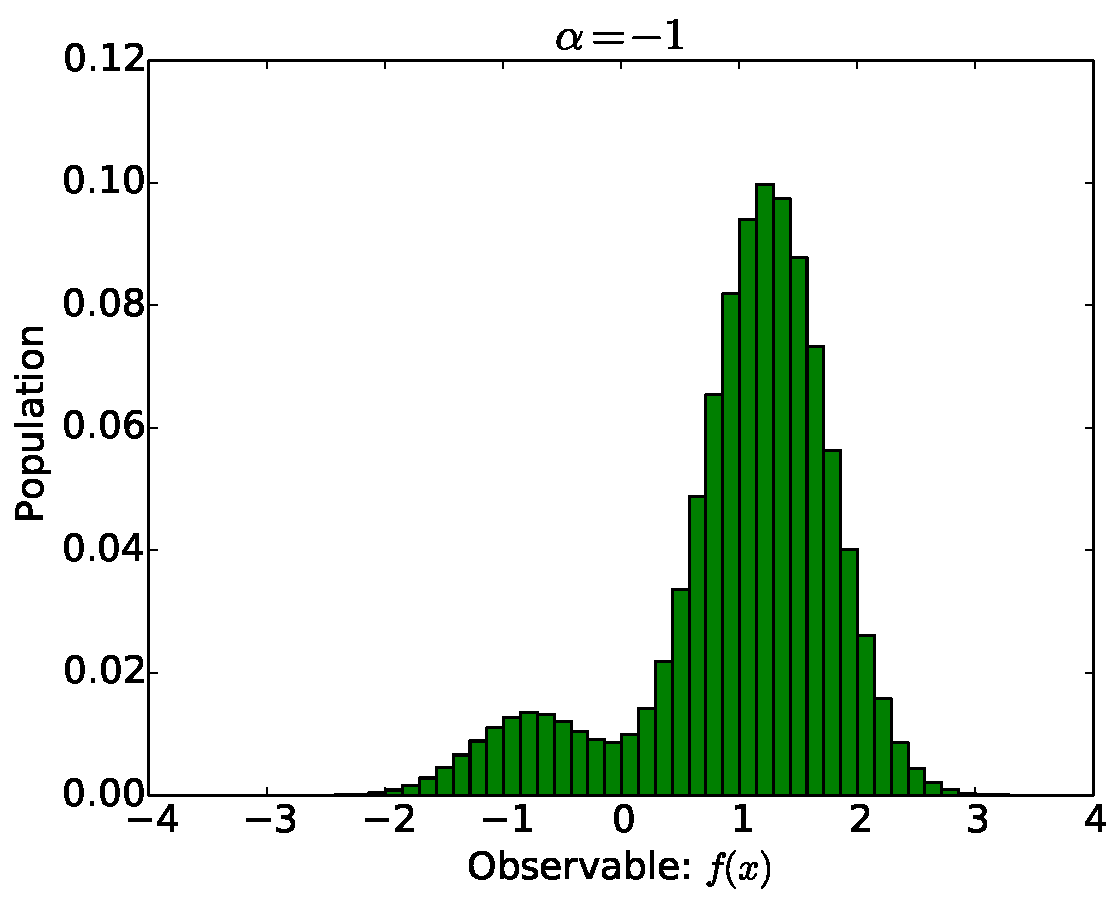
\includegraphics[width=5.0cm]{figures/model_hist-1.pdf}
}
\subfigure[]{
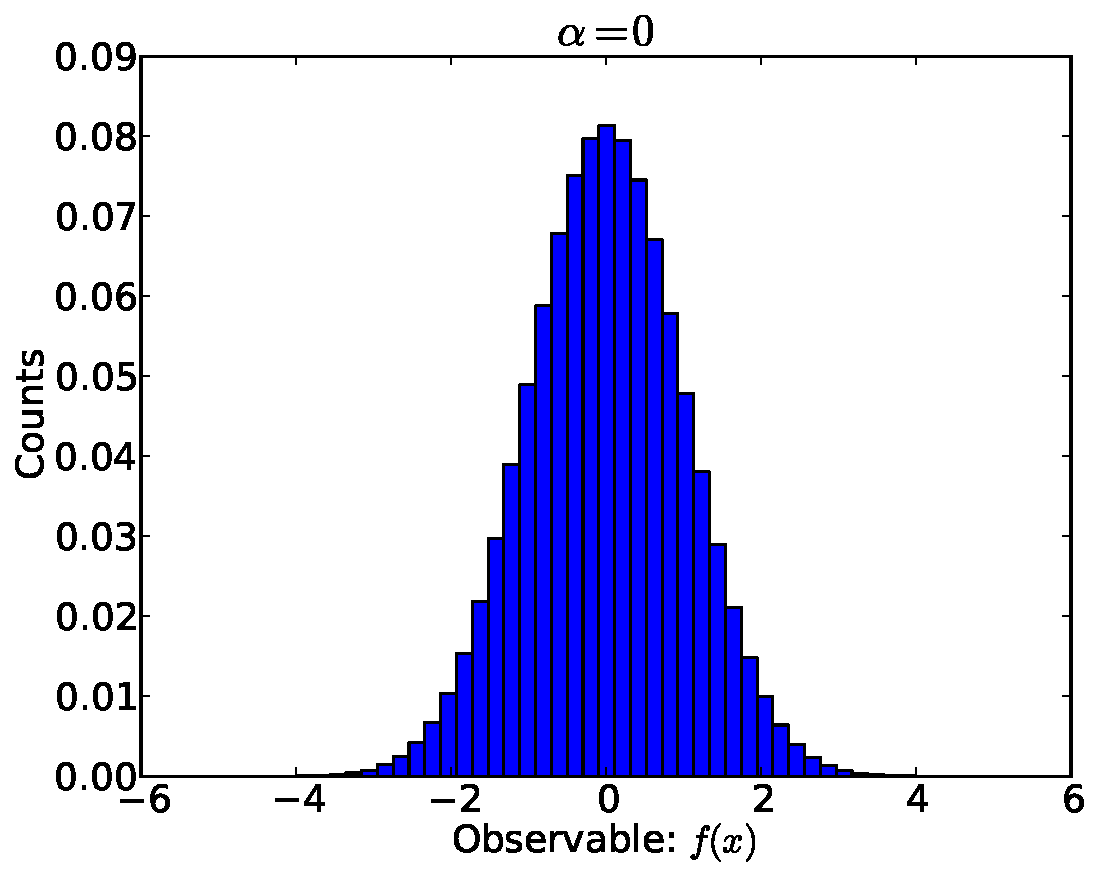
\includegraphics[width=5.0cm]{figures/model_hist0.pdf}
}
\subfigure[]{
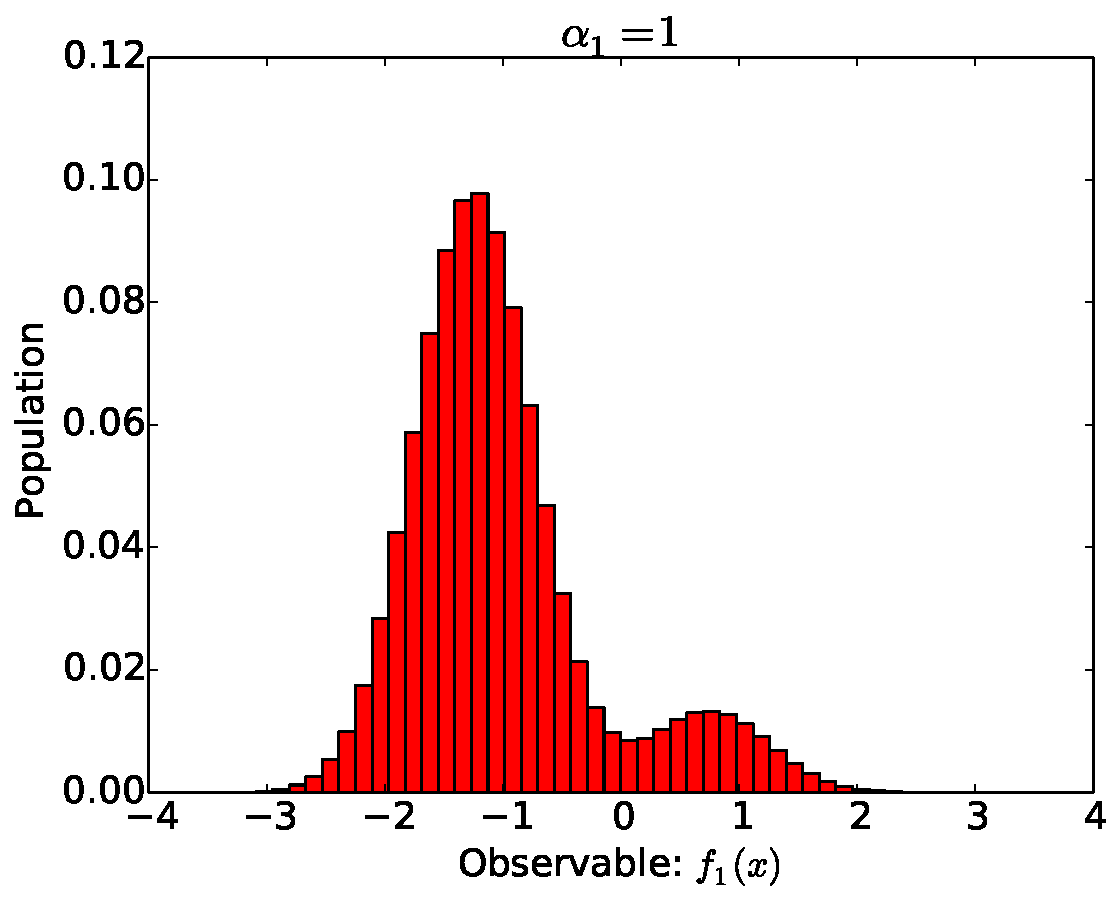
\includegraphics[width=5.0cm]{figures/model_hist1.pdf}
}

\subfigure[]{
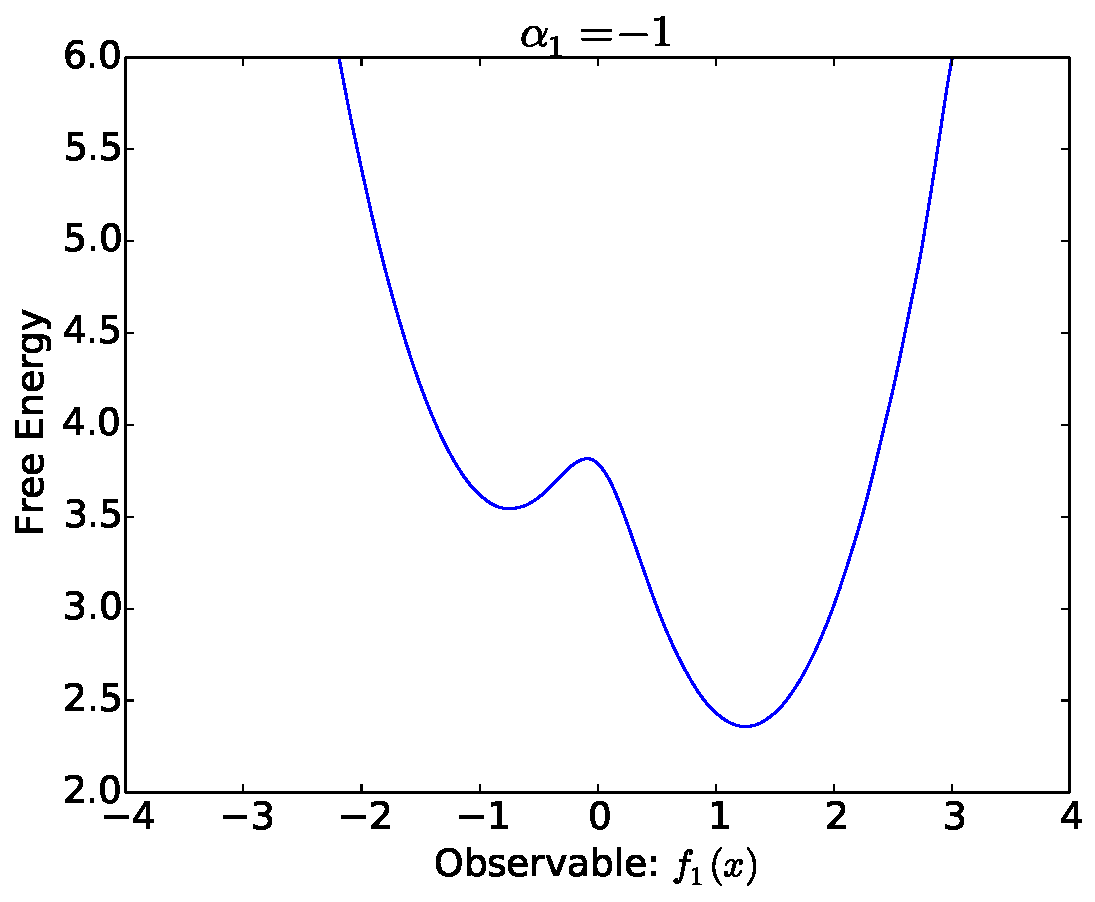
\includegraphics[width=5.0cm]{figures/model_landscape-1.pdf}
}
\subfigure[]{
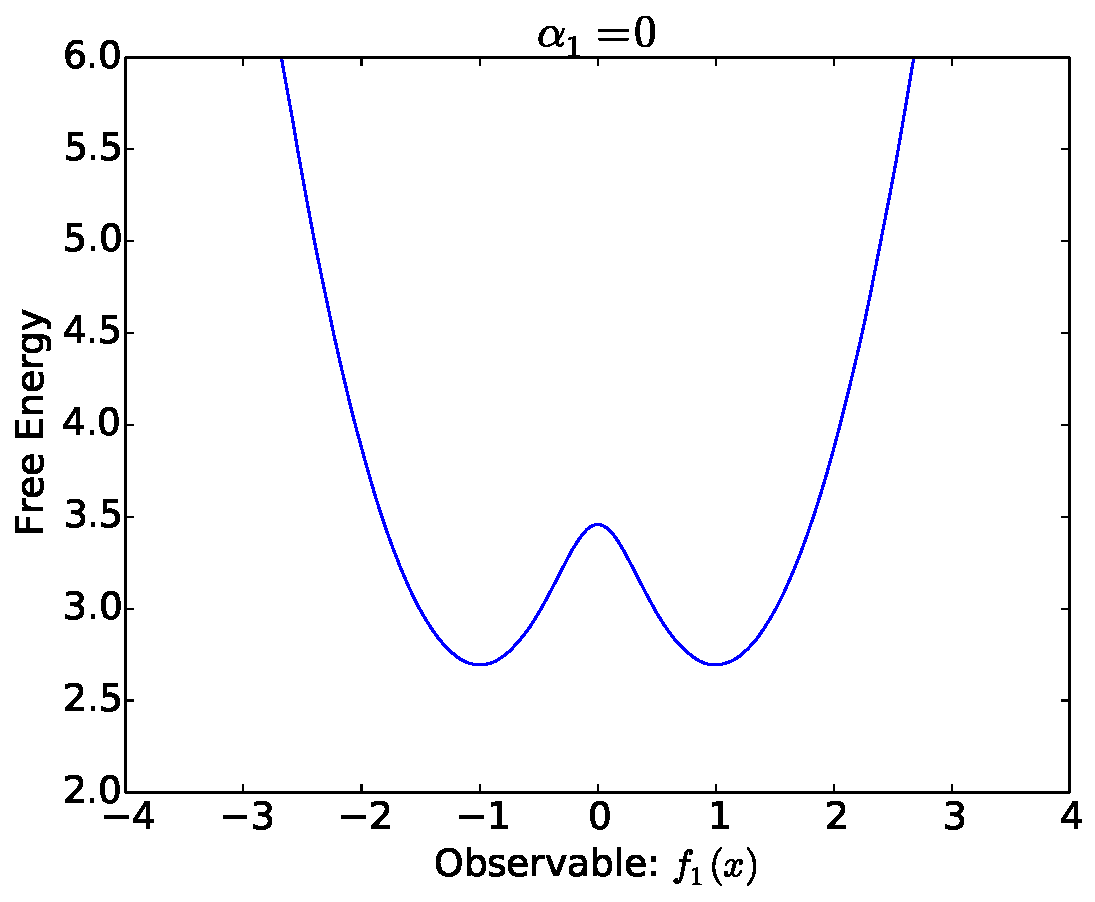
\includegraphics[width=5.0cm]{figures/model_landscape0.pdf}
}
\subfigure[]{
\includegraphics[width=5.0cm]{figures/model_landscape1.pdf}
}

\caption{
(a, b, c): Raw ($\alpha_1 = 0$) and reweighted (e.g. tilted) histograms of a one dimensional observable.  (d, e, f): The same, but plotted as free energies (e.g. $-kT \log(p)$).  
}
\label{figure:Hist}
\end{figure}



\subsection*{Connecting BELT and Maximum Entropy}


In BELT, we sample the following log posterior distribution:

$$LP(\alpha) = -\sum_i \frac{1}{2\sigma_i^2}(\langle f_i\rangle _\alpha - F_i)^2 + \log P(\alpha)$$

If we instead maximize the posterior probability, the problem becomes equivalent to setting the derivative of $LP$ to zero.  Assuming that the prior distribution is constant, the derivative is calculated to be the following:

$$ \frac{dLP}{d\alpha_k} =  -\sum_i \frac{1}{\sigma_i^2} (\langle f_i\rangle _\alpha - F_i) \frac{d\langle f_i\rangle _\alpha}{d\alpha_k} = 0$$

As before, if we find a value of $\alpha$ such that $\langle f_i(x) \rangle_\alpha = F_i$, we will maximize the posterior probability.  Thus, under ideal conditions, we expect similar results using the maximum entropy approach and BELT.  

\subsection*{Connecting BELT and Hyperensembles}

It has been argued \cite{crooks2007beyond} that a non-equilibrium ensemble $\rho$ ought to be characterized by the distance from equilibrium, as measured by the relative entropy.  Here we derive the BELT model using this entropic prior as a starting point.  In that work, Crooks defines a probability distribution on ensembles given by 

$$P(\rho) = \frac{1}{Z(\lambda)} \exp(- \lambda D(\rho || \rho^0))$$

In the above expression, $D(\rho || \rho^0)$ refers to the KL divergence of ensembles $\rho$ and $\rho^0$, while $\lambda$ is a parameter that characterizes the distance from equilibrium.  Note that the KL divergence, $D(\rho || \rho^0)$, can be expressed as a sum over the conformational states $j = 1, ..., m$:

$$D(\rho || \rho^0) = \langle \log(\frac{\rho}{\rho^0})\rangle_\rho = \sum_j \rho_j \log \frac{\rho_j}{\rho^0_j}$$

We let $\rho_0$ be a reference Boltzmann ensemble, which in our case will be simulation performed in a particular force field. Now, let us suppose that we have a single measurement $F$ that can be calculated via the ensemble average $\langle f(x) \rangle_\rho$.  Suppose that the likelihood of some measurement is given by

$$P(F|\rho) \sim N(\langle f\rangle_\rho, \sigma^2)$$

By Bayes' Theorem, we have that:

$$P(\rho | F) \propto P(F | \rho) P(\rho)$$

Letting $C$ be a normalizing constant, we have:

$$P(\rho | F) = C \exp(-\frac{1}{2\sigma^2} (\langle f \rangle - F)^2) \exp(-\lambda D(\rho || \rho^0))$$

For convenience, let $\phi$ denote the ensemble average, in the ensemble $\rho$, of the experimental observable of interest: 
$$\phi = \langle f \rangle_\rho = \sum_j f_j \rho_j$$

Suppose that $\rho^*(\phi)$ is the maximum entropy ensemble (in the sense of \cite{chodera2012}; see ``Outline of Maximum Entropy Formalism'') such that $\langle f \rangle_{\rho*} = \phi$.  The set of $\{ \rho^*(\phi)\}$ is a small subset of the set of all ensembles.  We now wish to see what happens when we integrate out or marginalize over the larger class of ensembles.  

We now wish to express the arbitrary ensemble $\rho$ as a perturbation from the maximum entropy ensemble $\rho^*(\phi)$.  We introduce a perturbation variable $\Delta_j = \rho_j - \rho^*_j$ and change variables from $\{\rho_j\}$ to ($\phi$, $\{\Delta_j \}$), where $\Delta$ is a correction to the maximum entropy ensemble $\rho^*(\phi)$.  We express the posterior probability in the new variables $\phi$ and $\Delta$:

$$P(\phi, \Delta | F) = C |J_1(\phi, \Delta)| \exp(-\frac{1}{2\sigma^2} (\langle f \rangle - F)^2) \exp(-\lambda D(\phi, \Delta|| \rho^0)) $$

In the above expression, $J_1(\phi, \Delta)$ is the Jacobian of the coordinate transformation.  With the above assumptions, the probability can be simplified:

$$P(\phi, \Delta | F) = C |J_1(\phi, \Delta)| \exp(-\frac{1}{2\sigma^2} (\phi - F)^2) \exp(-\lambda D(\phi, \Delta|| \rho^0)) $$

For a given value of $\phi$, $\rho^*(\phi)$ (e.g. $\Delta = 0$) maximizes the entropy.  This suggests a quadratic approximation to the entropy:

$$D(\phi, \Delta|| \rho^0) = \langle \log(\frac{\rho}{\rho^0})\rangle \approx D(\phi, 0|| \rho^0) + \frac{1}{2} \Delta^T H(\phi) \Delta$$

Here, $H_{ij}(\phi) = \frac{\partial^2 D}{\partial \Delta_j \partial \Delta_j}$, evaluated at the point of the maximum entropy ensemble $(\Delta = 0)$.  Inserting this expression in the probability gives:

$$P(\phi, \Delta | F) = C |J_1(\phi, \Delta)| \exp(-\frac{1}{2\sigma^2} (\phi - F)^2) \exp(-\lambda  D(\phi, 0|| \rho^0) - \frac{\lambda}{2} \Delta^T H(\phi) \Delta)$$

From the perspective of BELT, $\Delta$ is a nuisance parameter--we want an ensemble that is described by a more parsimonious representation.  We therefore integrate over $\Delta$ (e.g. marginalize) to achieve a probability that depends entirely on $\phi$.  

$$P(\phi | F) = C \int |J_1(\phi, \Delta)| \exp(-\frac{1}{2\sigma^2} (\phi - F)^2) \exp(-\lambda  D(\phi, 0|| \rho^0) - \frac{\lambda}{2} \Delta^T H(\phi) \Delta) d\Delta $$

$$P(\phi | F) = C \exp(-\frac{1}{2\sigma^2} (\phi - F)^2) \exp(-\lambda  D(\phi, 0|| \rho^0))  \int |J_1(\phi, \Delta)|  \exp(-\lambda \frac{1}{2} \Delta^T H(\phi) \Delta) d\Delta $$

For an analytically tractable calculation, $J_1(\phi, \Delta)$ must be independent of $\Delta$, so that we can remove it from under the integral.  To see that this is true, we first explicitly list all free parameters in the two representations.  In the $\rho$ representation, the free parameters are $\rho_1$, ..., $\rho_{m-1}$; $\rho_m$ can then be calculated as $\rho_m = 1 - \sum_{j=1}^{m-1} \rho_j$.  In the new representation, the free parameters are $\Delta_1, ..., \Delta_{m-2}, \phi$; the remaining terms can be calculated by noting that $\sum_j^m \Delta_j = 0$ and $\sum_j^m \Delta_j f_j = 0$.  The transformation between these coordinate systems is explicitly given by

$$\Delta_1 \rightarrow \rho_1 - \rho_1^*$$
$$...$$
$$\Delta_{m-2} \rightarrow \rho_{m-2} - \rho_{m-2}^*$$
$$\phi \rightarrow \sum_{j=1}^{m-1} \rho_i f_i + (1 - \sum_{j=1}^{m-1} \rho_j) f_n$$

This transformation is linear in $\rho_j$, so the Jacobian is constant.  The integral therefore simplifies as:

$$P(\phi | F) = C \exp(-\frac{1}{2\sigma^2} (\phi - F)^2) \exp(-\lambda  D(\phi, 0|| \rho^0)) |J_1|  \int   \exp(-\lambda \frac{1}{2} \Delta^T H(\phi) \Delta) d\Delta $$

The above expression requires integrating subject to the constraints $-\rho_j^*(\phi) \le \Delta_j \le 1 - \rho_j^*(\phi)$.  We assume that the likelihood is peaked around $\Delta=0$, so that the likelihood vanishes as we move far from $\Delta = 0$.  We can therefore replace the constrained integral to one over all space:

$$P(\phi | F) = C \exp(-\frac{1}{2\sigma^2} (\phi - F)^2) \exp(-\lambda  D(\phi, 0|| \rho^0)) |J_1|  \int_{-\infty}^\infty   \exp(-\lambda \frac{1}{2} \Delta^T H(\phi) \Delta) d\Delta_1 ... d\Delta_{m-2}$$


$$P(\phi | F) = C \exp(-\frac{1}{2\sigma^2} (\phi - F)^2) \exp(-\lambda  D(\phi, 0|| \rho^0)) |J_1|  \sqrt{(2\pi)^{m-2} \frac{1}{\lambda^{m-2} \det (H(\phi))}}  $$

To connect to BELT, we now change variables from $\phi$ to $\alpha$ (the tilting parameter of a BELT model), which introduces another Jacobian $J_2(\alpha)$

$$P(\alpha | F) = C \exp(-\frac{1}{2\sigma^2} (\langle f \rangle_\alpha - F)^2) \exp(-\lambda  D(\alpha, 0|| \rho^0)) |J_1|  |J_2(\alpha)|  \sqrt{(2\pi)^{m-2} \frac{1}{\lambda^{m-2} \det (H(\alpha))}}$$

To gain perspective in the comparison to BELT, we calculate the logarithm and drop all terms that are independent of $\alpha$:

$$\log P(\alpha | F) = -\frac{1}{2\sigma^2} (\langle f \rangle_\alpha - F)^2 -\lambda  D(\alpha, 0|| \rho^0) + \log |J_2(\alpha)| - \frac{1}{2} \log \det H(\alpha)$$

Assuming that our conformational samples were drawn from the Boltzmann ensemble $\rho^0$, the first two terms are identical to BELT with the maxent prior.  The remaining terms are corrections that account for the entropic cost of restricting our ensemble to be described by $\alpha$, rather than the entire space of possible ensembles.  The advantage of working with $\alpha$ is the dramatic reduction in the size of the parameter space.  In the limit of $\lambda \rightarrow \infty$ and $\sigma \rightarrow 0$ (and the approximations made above), the non-BELT terms vanish from the log likelihood.  

Another property to note is that the $\chi^2$ log likelihood is the only term dependent on $F$.  This implies that we can collect all the terms independent of $F$ and label them an effective prior:

$$\log P(\alpha | F) = -\frac{1}{2\sigma^2} (\langle f \rangle_\alpha - F)^2 + \log P_{eff}(\alpha)$$

Improved priors on $\alpha$ could possibly have the effect of correcting for the approximations (e.g. $\sigma\rightarrow 0$, $\lambda \rightarrow \infty$) used here in deriving BELT.  In practice, however, we found that deriving corrections to BELT using this approach did not lead to improved performance, possibly because of the simplifications used in the present derivation.  


\section*{Appendix S2.  Derivation of Reweighting}

Here we derive the population estimator used in BELT.  As in the main text, we use subscripted angle brackets to indicate ensemble averages in reweighted ensembles: $\langle h(x)\rangle _\alpha$ is the ensemble average of $h(x)$ in an ensemble that is perturbed by a biasing potential $\Delta (x;\alpha) = \sum_i \alpha_i f_i(x)$:

$$\langle h(x)\rangle _\alpha = \frac{1}{Z(\alpha)} \int h(x) dx \exp[ -U(x) - \Delta(x)]$$

$Z(\alpha)$ denotes the partition function for the $\alpha$ ensemble.  To proceed, we first note a simple Zwanzig identity that allows us to relate samples taken from different ensembles:

$$\langle h(x)\rangle _\alpha = \frac{1}{Z(\alpha)} \int h(x) dx \exp[ -U(x) - \Delta(x)] = \frac{Z(0)}{Z(\alpha)} \langle h(x) \exp[-\Delta(x;\alpha)]\rangle _0 $$

In the above expression, $\langle \rangle_0$ denotes an unperturbed ensemble (e.g. $\alpha = 0$) and $Z(0)$ is the partition function of the unbiased ensemble ($\alpha = 0$).  Now we sample from the unperturbed ensemble to statistically estimate the expectation

$$\langle h(x) \exp[-\Delta(x;\alpha)]\rangle _0 = \frac{1}{m} \sum_{j = 1}^{m} \exp [ - \Delta(x_j;\alpha)] h(x_j)$$

By letting $h(x) = 1$, we can estimate the partition function $Z(\alpha)$ up to the constant factor Z(0):

$$ \frac{Z(\alpha)}{Z(0)} = \frac{1}{m} \sum_j \exp[-\Delta(x_j;\alpha)]$$

Combining these equations, we have

$$\langle h(x)\rangle _\alpha = \sum_j h(x_j) \pi_j(\alpha)$$

where $\pi_j(\alpha)$ give estimates of the conformation weights at a particular value of $\alpha$:

$$\pi_j(\alpha) = \frac{1}{\sum_k \exp[-\Delta(x_k;\alpha)]} \exp[-\Delta(x_j;\alpha)]$$

Thus, BELT is essentially exponential averaging applied to a weighted combination of experiment-derived biasing potentials.  However, the present work has introduced two key advances.  First, the use of Markov chain Monte Carlo allows rigorous uncertainty analysis.  Second, regularization reduces the high variance previously associated with exponential averaging.  

\newpage

\section*{Appendix S3.  Alternative Error Models}

The model presented in the main text assumes independent normal deviations between measurements and the predicted ensemble.  This model is a useful approximation that leads to a straightforward $\chi^2$ likelihood.  However, in some situations, one might expect correlation between ensemble measurements.  Detecting this correlation would require additional experimental measurements.  However, it is possible to modify the $\chi^2$ likelihood to account for correlations between the predicted observables.  The net result is a modified log likelihood:

$$L L(\alpha) = \frac{1}{2} z^T P^{-1} z$$

where $P$ is the correlation matrix of the observables: $P_{ij} = Cor(f_i(x), f_j(x))$ and $z$ is the deviation between the $\alpha$ ensemble and the measurement, measured in units of the known uncertainty $\sigma_i$: $z_i = \frac{\langle f_i\rangle _\alpha - F_i}{\sigma_i}$.  Using this model will likely lead to increased estimates of uncertainties.  

Other possible error models involve modifying the assumption of normality.  A normal model penalizes models by the squared deviation from the experimental measurements.  However, expert knowledge may sometimes suggest different error models.  For example, one could imagine a model where small deviations are not penalized at all.  Such models could be inserted into the same MCMC framework with little extra effort.

\newpage

\section*{Appendix S4.  Choice of Prior}

\subsection*{Maximum Entropy (maxent) Prior}

As described in the main text, the maximum entropy prior is given by 

$$\log P(\alpha) = -\lambda \sum_j^m \pi_j(\alpha) \log \frac{\pi_j(\alpha)}{\pi_j^0}$$

Typically the reference populations are uniform; that is, $\pi_j^0 = \frac{1}{m}$.  This form of regularization has previously been used in a formalism for modeling SAXS ensembles \cite{rozycki2011saxs}.  

\subsection*{Dirichlet Prior}

We also consider the Dirichlet prior.  Dirichlet priors are commonly used as conjugate priors to multinomial random variables--that is, when dealing with counts and probabilities of categorical data.  The Dirichlet distribution is nonzero on the unit simplex and has the following functional form:

$$f(\pi;s) = \frac{1}{B(s)} \prod_j \pi_j^{s_j - 1}$$

In the above equation, $s$ is a vector of hyperparameters that are represent prior ``pseudocounts'' on frames, while $B(s)$ is a normalization constant containing a product of gamma functions:

$$B(s) = \frac{\prod_i \Gamma(s_i)}{\Gamma(\sum_i s_i)}$$

The Dirichlet prior is an obvious choice for BELT, because the object of interest is the probability distribution on conformations.  However, in BELT, we must restrict the distribution to the subset of probability distributions that can be achieved via reweighting.  Thus, instead of $\pi_j$, we have $\pi_j(\alpha)$:

$$f(\alpha;s) = \frac{1}{B(s)} \prod_j \pi_j(\alpha)^{s_j - 1}$$

For our MCMC calculations, we work with the $log$ probability:

$$\log f(\alpha;s) = -\log(B(s)) + \sum_j (s_j - 1) \log \pi_j(\alpha)$$

Note that the constant term is unimportant, as MCMC relies on the difference in $log$ probabilities:

$$\log f(\alpha;s) \approx \sum_j (s_j - 1) \log \pi_j(\alpha)$$

In practice, the Dirichlet prior has a large number of hyperparameters--the pseudocounts $s_i$ on each conformation.  To avoid the need for many hyperparameters, we assume that 

$$s_j - 1 = \lambda \pi_j^0$$

Thus, we assume that the pseudocounts are proportional to the raw MD simulation populations, which for constant temperature MD should be a uniform distribution.  For practical implementation in an MCMC sampler, we can drop terms that do not depend on $\alpha$, which leads to the following:

$$\log f(\pi;s) =  \lambda \sum_j \pi_j^0 \log \pi_j(\alpha)$$

Note that this can be rearranged into the following form, which better illuminates the connection between the maxent and Dirichlet priors:

$$\log P(\alpha) = -\lambda \sum_j \pi_j^0 \log \frac{\pi_j^0}{\pi_j(\alpha)}$$

Notice that this functional form is quite similar to the maxent prior that we previously discussed.  The difference between the maxent and Dirichlet priors can be explained in terms of the relative entropy between two distributions $P$ and $Q$.  The relative entropy is given by

$$D_{KL}(P||Q) = \sum_i P_i \log \frac{P_i}{Q_i}$$

The relative entropy is not a symmetric relationship--that is, $D_{KL}(P||Q) \ne D_{KL}(Q||P)$.  The maxent and Dirichlet priors are simply the relative entropy between $\pi(\alpha)$ and a reference distribution $\pi^0$, calculated in either direction.    For equilibrium molecular dynamics, the reference distribution is simply uniform ($\frac{1}{m}$).


\subsection*{Multivariate Normal (MVN) Prior}

In the MVN prior, $\alpha \sim N(\mu,\Sigma)$.  We let $\mu = 0$ to center the MVN around $\alpha = 0$.  This places the highest prior density on the raw simulation and allows regularization of $\alpha$.  To pick $\Sigma$, we note that the simple choice of $\Sigma_{ij} = \delta_{ij}$ leads to a prior that depends on the units of $\alpha$; this dependence on the unit system is undesirable.  However, if we choose $\Sigma_{ij} = \lambda Cov(f_i(x), f_j(x))$, the units of $\alpha_i$ and $f_i(x)$ cancel out in the MVN likelihood, leaving a result that is unit-invariant.  We have also introduced a scaling factor $\lambda$ to tune the amount of regularization.


\subsection*{Jeffrey's Prior}

Another choice of prior would be to use the Jeffrey's prior, which is uninformative and invariant under reparameterization.  We found Jeffrey's prior to be less desirable, however, because it does not necessarily place the prior maximum at $\alpha = 0$--thus, Jeffrey's prior was unable to provide regularization. 

\newpage

\section*{Appendix S5.  Determining Prior Strength Via Cross-Validation}

Each prior in this work contains a single free parameter, $\lambda$, which controls the level of regularization.  At least two different approaches can help select an appropriate value of $\lambda$:

\begin{enumerate}
 \item Cross validation on simulation data (used in main text)
 \item Cross validation on experimental data
\end{enumerate}

\subsection*{Cross validation on simulation data}

We first discuss cross-validating on the simulation data.  The underlying idea is that too little regularization ($\lambda = 0$) leads to models that overfit the available simulation data and generalize poorly--that is, repeating or extending the MD simulations would lead to a different result.  At the other extreme, underfit models ($\lambda = \infty$) will simply report the unbiased simulations, leading to poor agreement with experiment.  To perform this form of cross-validation, first separate the simulation data into several independent subsets.  Mark one subset as the ``test'' set and fit the model on the remaining data (the ``training'' set).  The $\chi^2$ score is evaluated on the test data.  We then repeat the process, letting the test set be equal to each of the other subsets.  The final $\chi^2$ square is averaged over each of these iterations.  The value of $\lambda$ is chosen to minimize the test set error.

When using MD to generate conformations, one must perform cross-validation using uncorrelated subsets of the data.  This precludes the typical standard cross-validation approach that uses randomly selected subsets of your data--randomly selected folds will be tainted by correlation between the folds.  As a thought experiment, suppose one cross validates by dividing your trajectory into even and odd frames.  Because of time-correlation in the data, the even and odd subsets will essentially contain the same information--ruining the cross-validation.  To avoid these perilous correlations, we recommend that you split the trajectory into time-contiguous blocks.  For the present work, we divided each trajectory into two halves.  

\subsection*{Cross validation on experimental data}

Cross validating on experimental data instead sets aside experimental measurements that can then be used to evaluate model quality.  One key difficulty with this approach, however, is that experimental datasets are often sparse--that is, there are often only few information-rich measurements.  This can lead to difficulties defining meaningful training and test sets.  

\subsection*{Cross Validation Results}

Here we summarize the values of $\lambda$ used in this work.  These values were determined by cross-validating on the simulation data.  

\vspace{5mm}

\begin{tabular}{lrrr}
\toprule
{}                &$\lambda$  &   &      \\
\midrule
prior &       MVN &  dirichlet & maxent \\
forcefield        &           &         \\
ff96           &      6.0  &    7.0  & 10 \\
ff99           &      1    &    1.25 & 4 \\
ff99sbnmr-ildn &      100  &    100  & 100 \\
charmm27          &      4    &   4     & 6 \\
oplsaa            &     12.0 &    13.0  & 15 \\
\bottomrule
\end{tabular}

\vspace{5mm}

The corresponding cross-validated reduced $\chi^2$ scores are given below.  These scores were generated using the training set of experimental measurements, but done in the setting of cross-validation on the simulation data.  Thus, the models were fit to half the trajectory data and evaluated on the other half.  As before, we see similar performance with all priors.  Full sweeps of $\lambda$ are depicted in Fig. \ref{figure:cross_val}.  To some extent, we expect similar performance between the priors.  This is because the relative entropy of normal distributions reduces to a weighted Euclidean distance between the means \cite{relative_entropy_wiki}.  However, the observables in the present work are non-normal, so the priors are not expected to give identical results.

For the amber99sbnmr-ildn results, cross validation recommends the use of large amounts of regularization.  This implies two things.  First, this forcefield is already in excellent agreement with experiment, so almost no reweighting is desired.  This may also indicate limitations in our estimates of the uncertainties in the chemical shifts and scalar couplings.  As a practical note, when large amounts of regularization are used, the resulting MCMC traces will contain essentially no variance.  It is thus necessary to use Bayesian Bootstrapping to get meaningful error bars.  For cases with less regularization, Bayesian Bootstrapping is less critical because the MCMC traces account for the majority of the uncertainty.

For ff99 with the maxent prior, we found that calculations with very low amounts of regularization suffer from occasional numerical instabilities.  Essentially, it appears that the regularization does not sufficiently penalize $\alpha_i \rightarrow \pm \infty$.

\vspace{5mm}


\begin{tabular}{lrrr}
\toprule
{} &  $\frac{1}{n}\chi^2$ (cross-validated) & &          \\
\midrule
prior &       MVN &  dirichlet & maxent  \\
forcefield        &           &  &       \\
ff96           &      0.39 &       0.37 &    0.39 \\
ff99           &      0.71 &       0.70 &    0.67 \\
ff99sbnmr-ildn &      0.35 &       0.35 &    0.34 \\
charmm27          &      0.62 &       0.59 &    0.54 \\
oplsaa            &      0.53 &       0.57 &    0.55 \\
\bottomrule
\end{tabular}

\newpage

\section*{Appendix S6.  Bayesian Bootstrapping}

The BELT model presented in the main text does not directly model simulation uncertainty.  This effect, however, can be introduced using a resampling technique known as Bayesian bootstrapping \cite{rubin1981}.  In Bayesian bootstrapping, every data point (e.g. conformation) is associated with a Dirichlet random variable that models the effect of resampling the given data points.  In effect, each conformation is given a ``prior'' population that is allowed to fluctuate around its average value of $\frac{1}{n}$.  

One additional complication arises when using molecular dynamics simulations, which produce a correlated time series.  Because of this, it is not sufficient to simply use a Dirichlet whose dimension is the same as the number of snapshots--such a procedure will significantly underestimate uncertainties due to correlation between frames.  Instead, one must first divide the trajectory into independent blocks.  The Dirichlet random variable is then chosen to sample the relative weights of each of the independent blocks.  Choosing the length of each block can be done by applying Bayesian bootstrapping to the un-reweighted trajectory.  Given some observable of interest, $O$, one calculates $O(B)$ for a sequence of block lengths, choosing the value of $B$ that maximizes the estimated uncertainty of $O$.  The block length could also be calculated using other blocking methods \cite{flyvbjerg1989error} or by statistical inefficiency analysis \cite{shirts2008}.  

In practice, applying Bayesian bootstrapping involves repeating several BELT calculations using different values of ``prior'' conformational populations that were drawn from a Dirichlet random variable.  The MCMC traces of each run are then pooled.  

\newpage

\section*{Appendix S7.  Convergence Analysis}

Although more sophisticated convergence tests are available, we evaluated convergence of MCMC traces by visual analysis.  A properly sampled and thinned model will appear similar to white noise, as observed in Fig. \ref{figure:MCMC}.  A few interesting features are worth noting.  The charmm27 and ff99 forcefields with MVN prior seem to suffer from increased correlation in their MCMC traces.  

Based on this and our other experience, we offer some suggestions for achieving converged traces.  First, it seems that the maxent and Dirichlet priors are better able to achieve independent MCMC samples than the MVN prior.  Second, poorer force fields (e.g. ff99, charmm27, and oplsaa) seem more prone to correlated MCMC samples.  This is likely because the sampler is forced to explore ``extreme'' models--that is, models that lie further from the raw forcefield.  Finally, we find that adding additional measurements--particularly ones that are correlated to previous measurements--leads to increased correlation within the MCMC traces.  We think these observations should help guide users towards achieving convergence without excessive computational resources.  

\newpage

\bibliographystyle{plain}
\bibliography{supporting_information}

\end{document}
